% Nejprve uvedeme tridu dokumentu s volbami
\documentclass[czech, master, public, dept460, male, cpdeclaration, oneside]{diploma}
% Dalsi doplnujici baliky maker
\usepackage{subfig}		% makra pro "podobrazky" a "podtabulky"
\usepackage{tikz}		% makra pro kresleni
\usepackage{float}   	% pro pozicovani obrazku
\usepackage{amsmath} 	% matice
\usepackage{fancyhdr}   % zahlavi
\usepackage{pgfplots}	% grafy

\ThesisAuthor{Marek Urban}
\CzechThesisTitle{Měření vzdáleností pro aplikace ve zpracování obrazu a shlukování}
\EnglishThesisTitle{Measuring the Distances for the Use in Image Processing and Clustering}
\SubmissionDate{24. dubna 2017}
\Thanks{Rád bych poděkoval doc. Dr. Ing. Eduardu Sojkovi za odbornou pomoc a konzultaci při vytváření této diplomové práce.}
\ThesisAssignmentImagePath{Figures/Assignment}
\AuthorDeclarationImageFile{Figures/AuthorDeclaration.jpg}
\CooperatingPersonsDeclarationImageFile{Figures/CoopPersonDeclaration.jpg}


\CzechAbstract{Práce se zabývá segmentací obrazu, především využitím různých metod měření vzdáleností v obrazových maticích a grafech. V první části textu uvedeme čtenáře do problematiky digitálního obrazu. Následně se zaměříme na formální definici pojmů metrika, vzdálenost a shlukování. Po definování potřebné teoretické pojmologie si vysvětlíme segmentaci obrazu jakožto speciální případ shlukování.\par
Následující kapitola se zabývá samotnou problematikou měření vzdáleností, detailně jsou vysvětleny rozdíly mezi euklidovskou, geodetickou a rezistivní vzdáleností, kde u každé jsou vyzdviženy výhody a nevýhody. V závěru textu se podíváme na implementaci experimentu dle definované teorie, a rozebereme si dosažené výsledky v jednotlivých definovaných scénářích.
}

\CzechKeywords{shlukování, segmentace obrazu, spektrální shlukování, metrika, vzdálenost, měření vzdáleností, analýza obrazu, počítačové vidění, euklidovská vzdálenost, rezistivní vzdálenost, geodetická vzdálenost}

\EnglishAbstract{The main interest of this thesis is to examine methods for measuring distances in image segmentation algorithms. The first lines of this text we will introduce reader to the problematics of digital imagery. Next we will focus on formal definitions of terms like metric, distance and clustering. After defining the necessary terminology we will dive into the image segmentation topic as a specific case of data clustering. \par
The next chapter will be describing the problems behind measuring distances in segmentation algorithms. Euclidean, geodesic and resistance distances are described in detail with specific advantages and problems. In the final chapters text is focused mainly on the experiment which was build according to described theory. Last chapter is examining the results achieved in specific scenarios.   
}

\EnglishKeywords{clustering, image segmentation, spectral clustering, metric, distance, measuring distances, image analysis, computer vision, euclidean distance, resistance distance, geodesic distance}

\AddAcronym{EV}{Euklidovská vzdálenost}
\AddAcronym{GV}{Geodetická vzdálenost}
\AddAcronym{RV}{Rezistivní vzdálenost}
\AddAcronym{RGB}{Red Green Blue}
\AddAcronym{DA}{Dijkstrův algoritmus}
\AddAcronym{U}{Elektrické napětí}
\AddAcronym{I}{Elektrický proud}
\AddAcronym{R}{Elektrický činný odpor}
\AddAcronym{KZ}{Kirchhoffův zákon}
\AddAcronym{$F_{MS}$}{Mumford-Shahův funkcionál}
\AddAcronym{LoG}{Laplacian of Gaussian}

% Zacatek dokumentu
\begin{document}
	
% Nechame vysazet titulni strany.
\MakeTitlePages
% Pokud mame v zaverecne praci vypisy kodu, jinak odstranit.
\lstlistoflistings

% A nasleduje text zaverecne prace.
\section*{Úvod}
Jako je již dobrým zvykem i tato práce se v první části bude zabývat především popisem problematiky samotné. Jak již bylo zmíněno výše, práce se zabývá analýzou obrazu, především tedy obrazovou segmentací. Procesem obrazové segmentace myslíme rozdělení pixelů digitálního obrazu do skupin. Shluky vytvořené segmentačním algoritmem by si v ideálním případě měly být podobné. Podobností můžeme myslet například podobnou barvu, jas nebo například tvar. Vlastnosti určené k porovnávání nazýváme momenty. Důležitý je ovšem fakt, že všechny shlukovací algoritmy nějakým způsobem podobnost mezi jednotlivými objekty vyčíslují. Pro segmentaci obrazu existuje velké množství algoritmů, jejichž popisem se budeme ve zkratce zabývat později.\par
Obecný název pro tyto algoritmy se nazývá shluková analýza. Algoritmy shlukové analýzy využívají různé metody měření vzdáleností mezi počáteční (referenční) hodnotou a měřeným bodem. Velice častým způsobem pro měření vzdáleností je vzdálenost euklidovská. Ta ovšem přes svou jednoduchou a přímočarou implementaci má jisté nevýhody, které si do detailu rozebereme níže. Cíl této práce je porovnání právě euklidovské vzdálenosti s jinými více pokročilými metodami měření vzdálenosti, jako je například vzdálenost geodetická či rezistivní. Porovnání těchto metrik si ukážeme právě na shlukovacích algoritmech pro segmentaci obrazu.\par
Segmentace obrazu je bezpochyby velice důležitou částí algoritmů obrazové analýzy a strojového vidění celkově. Cílem segmentace obrazu je vyseparování částí obrazu od pozadí nebo alternativně rozdělení částí obrazu podobnými momenty do skupin. I přestože je této problematice věnována velká pozornost výzkumných týmů z celého světa, problém segmentace obrazu stále není plně vyřešen. Problém nastává již ve chvíli máme-li jasně definovat, jak má segmentovaný obraz vypadat. Segmentační algoritmy lze nastavit s mnoha prahovými hodnotami, které ovlivňují výsledný počet a tvar shluků. Není ovšem nijak definováno kolik by shluků mělo být případně jak mají být velké. Práce se bude pokoušet odpovědět na otázku, které měření vzdáleností je nejlepší ve specifických případech.
\begin{figure}[H]
	\vspace*{+3.0mm}
	\centering
	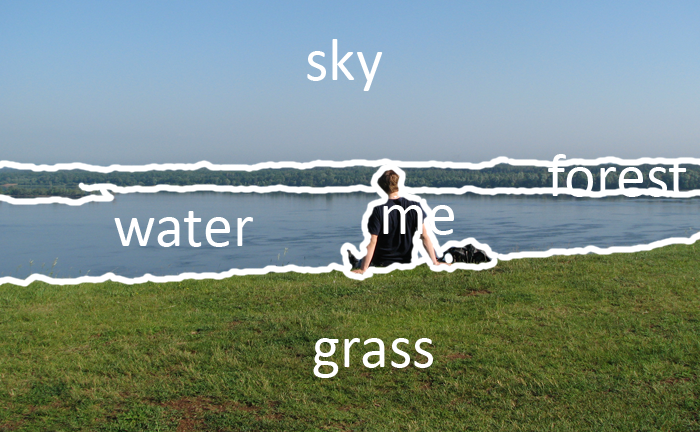
\includegraphics[height=5cm]{Figures/explanatory/1-segmentation.jpg}
	\caption{Ukázka segmentace obrazu}
\end{figure}

\section{Reprezentace obrazu}
Práce se bude zabývat analýzou obrazu a počítačovým viděním, i přestože pro nás lidi je pojem obrazu jasnou záležitostí, není od věci definovat si pojmy jako obrazová funkce a následně si osvětlit její reprezentaci v počítačové paměti.

\pagestyle{fancy}
\fancyhf{}
\headsep = 15pt
\renewcommand{\sectionmark}[1]{\markright{\arabic{section}.\ #1}}
\fancyhead[R]{\rightmark}
\renewcommand{\headrulewidth}{1pt}
\fancyfoot[C]{\thepage}

\subsection{Obrazová funkce}
Jedná se o teoretický předpis popisující spojitý obraz. Máme-li spojitou funkci $f(x)$ můžeme na ni nahlížet jako na reprezentaci jednorozměrného spojitého obrazu. Obraz ovšem ve své klasické podobně mívá jak šířku tak výšku. Z tohoto tedy výplývá obrazová funkce dvourozměrná. Tu můžeme definovat jako $f(x,y)$ kde $x$ a $y$ jsou proměnné reprezentující horizontální a vertikální souřadnice v obrazu. \cite{Sojka} \par
Spojité funkce mají ovšem pro výpočetní techniku velice nemilou vlastnost, tou je fakt, že i na konečném intervalu obsahují nekonečné množství hodnot. Je tedy bežnou praxí provedení diskretizace původní obrazové funkce. Diskretizací rozumíme proces, kdy nekonečně ''jemnou'' spojitou funkci rozdělíme na stejně velké vzorky (samply) reprezentující vzorkovaný interval.\par
Vzorkováním obrazu pochopitelně vždy dochází ke ztrátě původní informace. Se zvětšujícím se vzorkovacím intervalem také dochází k růstu zkreslení původního obrazu (například kruh se více a více přibližuje čtverci). Se zvyšujícím se výkonem počítačů a růstem kapacity paměťových médií je možné vzorkovací interval snižovat a tedy zvyšovat všobecnou kvalitu digitalizovaného obrazu. 

\begin{figure}[H]
	\vspace*{+3.0mm}

	\centering	
	\subfloat[Originální obraz]{{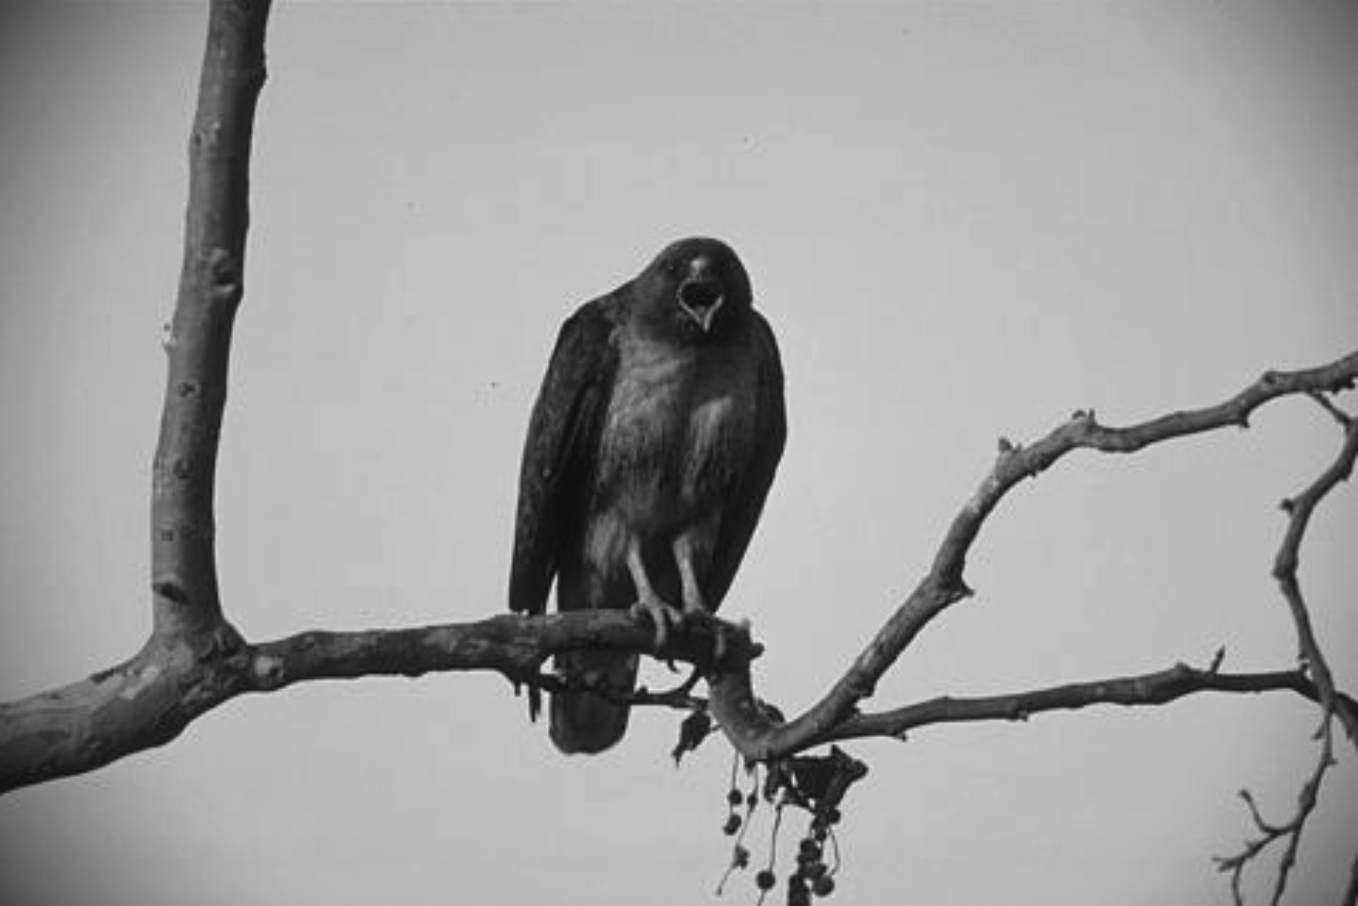
\includegraphics[width=6.5cm]{Figures/explanatory/bird-ori.png} }}
	\subfloat[Diskretizovaná obrazová funkce]{{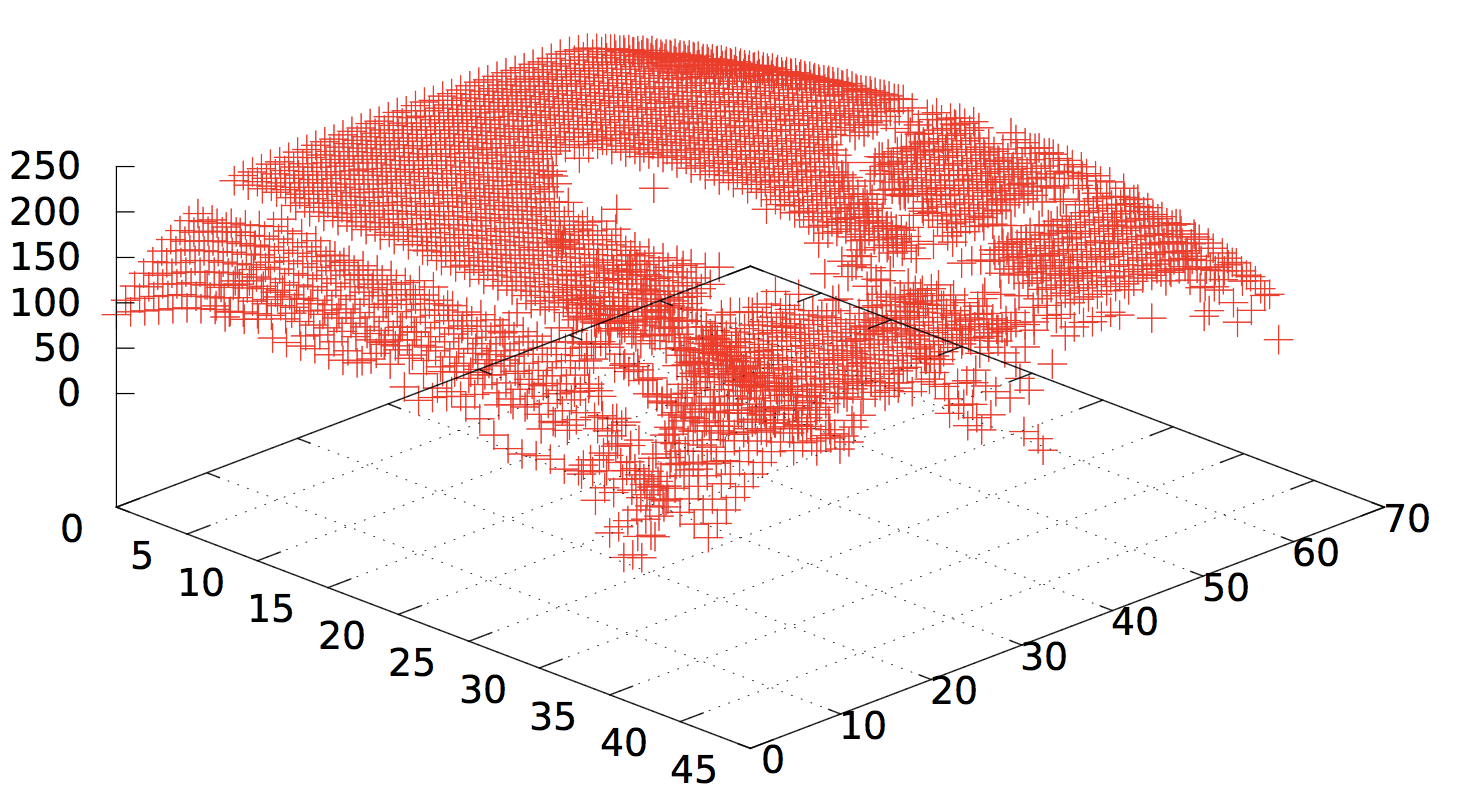
\includegraphics[width=6.5cm]{Figures/explanatory/bird-function.png} }}
	\qquad
	\caption{Reprezentace obrazu \cite{Cima}}
\end{figure}
\subsection{Digitální obraz}
Digitalní obraz vzniká digitalizací (vzorkováním) obrazové funkce. Jelikož obrazová funkce je dvourozměrná, digitální obraz je taktéž reprezentován pomocí dvourozměrného rastru. Prvku rastru říkáme pixel, neboli obrazový bod. Pixel samotný může být reprezentován jedinou hodnotou nebo případně celým vektorem hodnot. U černobílých obrazů je postačující jasová informace pixelu, ta může být v extrémním případě pouze jednobitová (binární obraz), kde obraz je složen pouze z absolutní černé a absolutní bílé. Ve většině případů ovšem požadujeme, aby informace mohla obsahovat více než dvě barvy (resp. odstíny šedi). \par
Zdaleka nejrošířenější bývají právě 8-bitové obrazy, kde hodnota pixelu je daná 8-bitovou informací, hodnoty jasu mohou tedy nabývat hodnot 0 - 255. U dražší, zpravidla profesionální techniky je bežné, že obrazy bývají 12-bitové což umožňuje zaznamenat 8x větší jemnost jasového přechodu. U vědeckých nástrojů nejsou vyjímkou ani 16-bitové kamery, schopné zachytit až 65 536 jasových úrovní. \par
Popis výše samozřejmě hovořil o případu, kdy obrazový pixel je definován pouze jedinou hodnotou. V takovémto případě se většinou jedná právě o černobílý obraz (rozumíme obraz v odstínech šedi). O tomto obraze říkáme, že se jedná o obraz jednokanálový. Všichni dobře známe obrazy barevné, k dosažení barevného efektu se zpravidla používá RGB barevný model. Jednokanálový obraz je rozšířen na obraz tříkanalový. Každý kanál drží informace o intenzitě jedné z RGB složek. Současné technologie digitálních snímačů nedokáží rozpoznat míru barevného spektra dopadající na snímač pouze celkovou intenzitu. K získání individuálních hodnot jednotlivých barev je dosaženo pomocí Bayerova filtru \cite{Bayer}, alternativou jsou tříčipové kamery využívající třech nezávislých senzorů, na které dopadá světlo barevně roptýlené krystalickým členem.
\begin{figure}[H]
	\vspace*{+3.0mm}
	\centering
	\subfloat[Bayerův filter]{{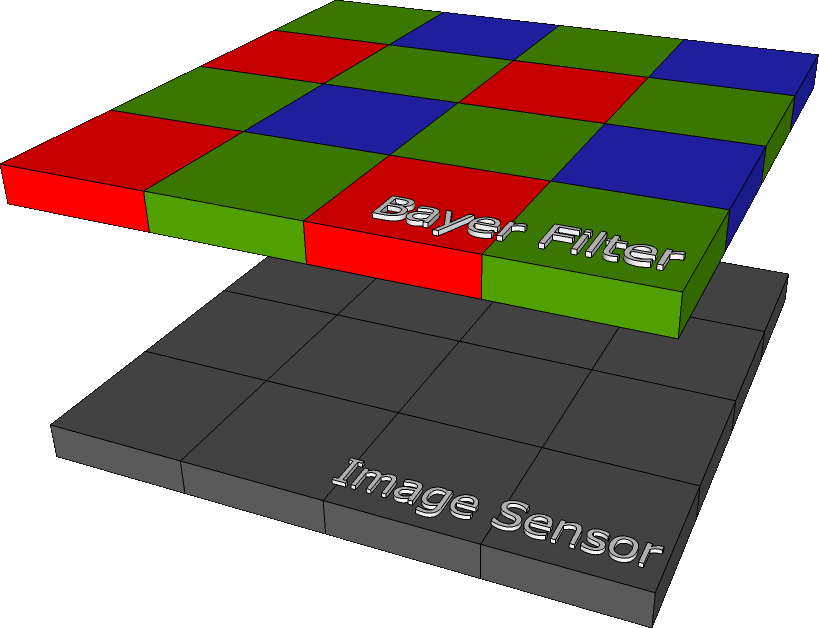
\includegraphics[width=5.5cm]{Figures/explanatory/bayerfilter.png} }}
	\subfloat[RGB rozklad krystalem]{{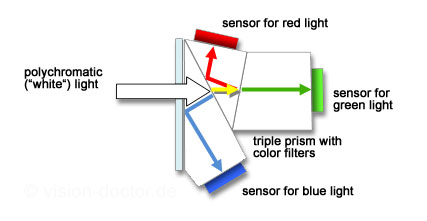
\includegraphics[width=8.5cm]{Figures/explanatory/colorPrism.jpg} }}
	\qquad
	\caption{Metody získávání barevného obrazu}
\end{figure}

\noindent
Součástí obrazových pixelů nemusí být nutně jen viditelné informace. Stále častěji se objevují senzory s možností měřit vzdálenost daného bodu v době expozice (RGB-D). Hloubková informace pixelu, může být taktéž použita pro rozpoznání objektů v obraze.\par
Nyní rozumíme problému, že obraz je z pohledu počítače pouze množina bodů (pixelů) bez jakéhokoliv definovaného kontextu. Úkolem segmentace je pokusit se nalézt body s podobnými vlastnostmi a správě je zařadit do segmentů dle definované podobnosti.

\section{Vzdálenost a shlukování}
Dříve než se položíme hlouběji do tématu segmentace obrazu, je zapotřebí si definovat, co je vlastně vzdálenost a segmentace z abstraktního hlediska. Hlavním cílem práce je především zmapování různých metod pro měření vzdáleností v obraze a jejich využitelnost pro obrazovou segmentaci. Je tedy důležité si formálně definovat pojem vzdálenosti, metriky a shlukové analýzy.

\subsection{Metrický prostor}
Metrický prostor je definován jako dvojice $(M, p)$, kde $M$ je libovolná neprázdná množina a $p$ je metrika.

\subsection{Metrika}
Je zobrazení splňující tyto axiomy (pro libovolná $x, y, z \in M$):
\begin{enumerate}
	\item Axiom nezápornosti $p(x,y) \geq 0$
	\item Axiom totožnosti $p(x, y) = 0 < == > x = y$
	\item Axiom symetrie $p (x, y) = p (y, x)$
	\item Trojúhelníková nerovnost $p(x,z)  \leq p (x,y) + p(y,z)$
\end{enumerate}

\subsection{Vzdálenost}
Pojmy vzdálenost a metrika se v běžné hovorové komunikaci používají záměnně. Nicméně z formálního hlediska se nejedná o totéž. Z definice metriky vidíme, že metrika je pouze zobrazení splňující dané axiomy, může se tedy jednat i zobrazení jiné než vzdálenost v klasickém slova smyslu.\par
Vzdálenost na druhou stranu, by šlo pospat jako podmnožinu pojmu metrika. Tedy každá vzdálenost je metrikou, ale ne naopak. Analyzujeme-li co empiricky chápeme pod pojmem vzdálenost, dostaneme právě axiomy metriky. Je zřejmé že vzdálenost mezi dvěma body je vždy nezáporná (axiom nezápornosti). Nulová je pouze v případě, jsou dva porovnávané body totožné (axiom totožnosti). Taktéž nás nepřekvapí fakt, že vzdálenost z místa A do místa B je stejná jako vzdálenost z místa B do místa A (axiom symetrie). Při promyšlení je i zřejmé, že cesta z A do B a pak do C není kratší než cesta z A přímo do C (trojúhelníková nerovnost). \cite{Shlukovani}

\subsection{Využití v segmentaci obrazu}
Všechny shlukovací algoritmy v jisté části svého běhu provádějí rozhodování, zda daný pixel do shluku (segmentu) náleží či nikoliv. Hodnota pixelu se porovnává s jinou hodnotou reprezentující daný segment. V principu se tedy provádí měření vzdálenosti mezi porovnávaným pixelem a referenční hodnotou. 

\subsection{Shluková analýza}
Segmentace obrazu je speciálním případem shlukování. Problémem shlukování se obecně zabývají metody shlukové analýzy. Jedná se o tzv. metody učení bez učitele. Cílem těchto metod na dané množině objektů nalézt její podmnožiny – v našem případě segmenty v obraze. U vytvořených podmnožin samozřejmě očekáváme podobnost a současně jednotlivé podmnožiny jsou navzájem disjunktní. Formálně lze rozklad popsat pomocí množiny  a její neprázdných podmnožin. \cite{Shlukovani}

\begin{equation}
\vspace*{+3.0mm}
\Omega = {C_1, C_2, C_3, ... C_n}
\end{equation}

\begin{equation}
\vspace*{+3.0mm}
C_i \cap C_j = \emptyset
\end{equation}

\begin{equation}
\vspace*{+3.0mm}
C_1 \cup C_2 \cup ... \cup C_n = \Omega
\end{equation}

\subsection{Hierarchické a nehierarchické shlukování}
Algoritmy shlukové analýzy se dají rozdělit na hierarchické a nehierarchické. Hierarchické shlukování se dá definovat jako sekvence vnořených rozkladů, kde na začátku jsou všechny prvky množiny jednoprvkový shluk a průběhem shlukování se jednotlivé prvky spojují, až do stavu kdy dostaneme shluk jediný obsahující všechny objekty. Toto se nazývá shlukování aglomerativní, existuje i shlukování divizní, které naopak začíná jediným shlukem a provádí rozklad až do situace kdy všechny shluky jsou jednoprvkové.\par
Druhým typem jsou právě algoritmy nehierarchické. Nevytvářejí hierarchickou strukturu, rozkládají danou množinu do podmnožin dle předem daného kritéria. Hlavní rozdíl oproti hierarchickým metodám je fakt, že pro provedení původního rozdělení (resp. spojení) už další krok rozdělení neprovádíme. Výsledkem jsou tedy disjunktní podmnožiny. Právě touto skupinou algoritmů se budeme zabývat pro řešení obrazové segmentace. \cite{Kumar}

\section{Segmentace obrazu}
Segmentací obrazu rozumíme postup při, kterém se snažíme z individuálních pixelů vytvořit regiony, které spolu souvisí. Obecně lze říci,  že se jedná o náročný případ shlukování. Náročný proto, že obrazová data mohou být různě složitá a často jsou do jisté míry poškozena šumem. V dnešní době existuje celá řada algoritmů snažících se řešit problematiku obrazové segmentace. V jádru věci, ale všechny rozhodují, zda daná dvojice bodů náleží do stejného segmentu či nikoliv. K rozhodnutí této otázky je zapotřebí najít metodu k vyčíslení podobností těchto tvou bodů. K tomuto účelu slouží právě metody pro měření vzdáleností. 

\subsection{Neurčitý výsledek}
Určení správné výsledné segmentace je znatelný problém. Faktem je, že žádná ideálně správná segmentace obrazu obecně neexistuje. Výsledek segmentace (velikost a počet segmentů) je závislý na nastavení prahů při běhu algoritmu. Tyto prahy definují, v jaké chvíli je naměřená vzdálenost ještě považována za součást segmentu a kdy se již jedná o segment jiný. V následující ukázce můžeme vidět segmentovaný obraz za použití různě "přísných" thresholdů. Je evidentní, že ani samotní lidé se nemusí shodnout, která segmentace je správná. Ideální nastavení prahu je spíše závislé na konkrétní situaci a problému, který se snažíme řešit. Nicméně ani tento fakt nezbránil výzkumníkům v pokusu o nalezení formálního zápisu segmentace. \cite{Gaura}

\begin{figure}[H]
	\centering	
	\subfloat[Originál]{{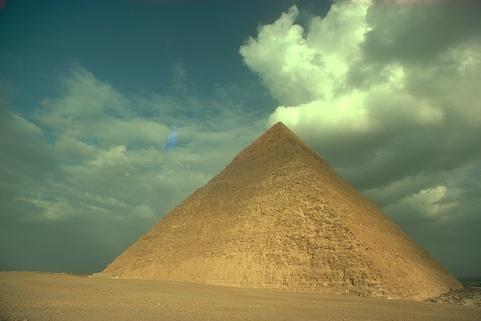
\includegraphics[height=4.0cm]{Figures/explanatory/2-segm-ori.jpg} }}
	\subfloat[Vysoký práh]{{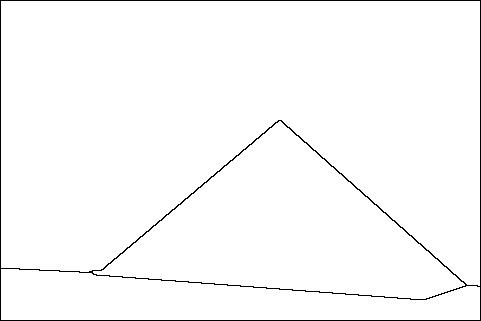
\includegraphics[height=4.0cm]{Figures/explanatory/2-segm-hi-t.jpg} }}
	\qquad	
	\subfloat[Střední práh]{{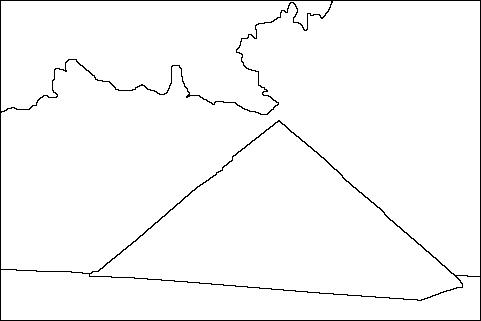
\includegraphics[height=4.0cm]{Figures/explanatory/2-segm-med-t.jpg} }}
	\subfloat[Nízký práh]{{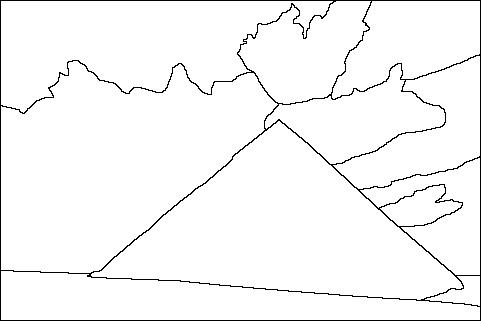
\includegraphics[height=4.0cm]{Figures/explanatory/2-segm-low-t.jpg} }}
	\caption{Různé výsledky segmentace \cite{Berkeley}}
\end{figure}

\subsection{Věta o nemožnosti}
Problém nalezení univerzálního postupu v segmentaci obrazu byl v roce 2002 formulován profesorem Jonem Kleinbergem. Hlavní poentou jeho práce vysvětlení, proč žádná obecná metoda pro segmentaci obrazu nemůže existovat. Podle Kleinbergera by takováto metoda měla splňovat tři vlastnosti a to stálost, bohatost a neměnná vůči změně měřítka. \cite{Kleinberg} \par
Máme množinu $S$ značící vstupní data v podobě obrazové matice. $\Omega$ je rozklad množiny $S$ pomocí shlukovací funkce $f(d)$. Množina  $range(f)$ má význam všech možných rozkladů $\Omega$ pro libovolnou distanční funkci  $d$. Definování těchto množin a funkcí je důležité pro formální zápis axiomů pro větu od nemožnosti.

\subsubsection{Stálost}
Anglicky, \textit{Consistency} popisuje vlastnost, při které pokud zmenšíme vzdálenosti mezi prvky jednotlivých shluků a zvětšíme vzdálenost mezi jednotlivými shluky, měli bychom dostat stále stejnou segmentaci.
\begin{definition}
	Pokud zmenšíme vzdálenosti mezi členy uvnitř shluku $C_k$ a zvětšíme vzdálenosti mezi
	jednotlivými shluky $C_1, C_2...C_n$ měly bychom dostat stejný rozklad množiny $S$.
\end{definition}

\subsubsection{Bohatost}
Anglicky \textit{Richness}, pro libovolný rozklad $\Omega$ je možno nalézt distanční funkci $d$, takovou že $f(d) = \Omega$.
\begin{definition}
	$range(f)$ se rovná množině všech možných rozkladů $S$
\end{definition}

\subsubsection{Neměnnost}
Respektive neměnnost vůči změně měřítka, anglicky \textit{Scale-Invariance}. Shlukovací funkce $f(d)$ nesmí být citlivá ne změnu jednotkové míry, respektive měřítka distanční funkce.
\begin{definition}
	Pro libovolnou distanční funkci $d$ a nějaké $a : a > 0, a \in R$, platí $f(d) = f(a * d)$.
\end{definition}

\subsubsection{Definice}
Nyní si můžeme definovat Kleinbergovu větu o nemožnosti. Existuje-li množina $S = {x_1, x_2, ... x_n} \wedge |S|  \geq 2$, tak k ní neexistuje žádná segmentační funkce $f(d)$, která by byla zároveň bohatá, stálá a neměnná vůči změně měřítka.\par
Není potřeba nadále hlouběji prozkoumávat jednotlivé axiomy, jelikož již máme matematickou větu definující hypotézu neexistence univerzální shlukovací funkce. Přestože jsme nyní definovali, že nalezení obecné segmentační funkce je nemožné, nabízí se cesta sledování kvality výsledklů, již existujících specifických shlukovacích funkcí.

\subsection{Mumford-Shahův funkcionál}
O obecný popis problému obrazové segmentace se taktéž v roce 1989 pokusili výzkumníci David Mumford and Jayant Shah. Přišli s velice uznávanou definicí pro obrazovou segmentaci. Problém pospali jako minimalizaci jejich Mumford-Shahova funkcionálu. \cite{Mumford}

\begin{equation}
\vspace*{+3.0mm}
 F_{MS}(f(x), B) =  \alpha \int_{\Omega} [g(x) - f(x)]^2 dx + \beta  \int_{\frac{\Omega}{\beta}} |\bigtriangledown f(x)|^2 dx + \gamma |\beta|
\end{equation}
Funkce $g(x)$ nám reprezentuje originální obraz, $f(x)$ je výsledný obraz mající minimalizovat funkcionál. Symbol $\Omega$ je plocha našeho obrazu. $B$ je množina hraničních bodů mezi oblastmi v obraze, $\alpha, \beta, \gamma$ jsou váhy určující chování funkcionálu a vlastnosti výsledné segmentace.\par
Funkcionál $F_{MS}$ definuje kritéria pro optimální segmentaci obrazu a je využíván například v level-set metodách. Detailnějším popisem těchto metod se nebudeme dále zabývat, abychom nerozváděli práci do témat, které s prací přímo nesouvisí. Minimalizací funkcionálu můžeme ovšem ukázat zajímavý vztah mezi $F_{MS}$, spektrálním shlukováním a Laplaceovou maticí.\par
Po vyřešení minimalizace $F_{MS}$ dostaneme:
\begin{equation}
\vspace*{+3.0mm}
\beta \min\limits_{f(x,y)}  \int_{\frac{\Omega}{\beta}} (\bigtriangledown f(x, y))dS \Longleftrightarrow \beta \bigtriangledown f(x,y) = 0
\end{equation}
\begin{definition}
	Vztah 5 bude mít minimální řešení právě tehdy, když Laplaceův diferenciální operátor $\bigtriangledown$ na funkci $f(x, y)$ bude roven 0.
\end{definition}
Jinými slovy lze říci, že řešení minimalizace existuje pouze pro takové funkce $f(x,y)$, které jsou řešením homogenní Laplaceovy rovnice. \cite{Pecha}
\subsection{Algoritmy pro segmentaci obrazu}
Výzkum obrazové segmentace probíhá již mnoho let, za tuto dobu bylo již vyvinuto stovky metod řešící tento problém. Nicméně, stále neexistuje žádná perfektní metoda vhodná pro řešení libovolného problému. Stejně tak se nedá říci, že různé metody poskytují podobně kvalitní výsledky na různých obrazech. Nalezení obecného postupu pro volbu správného segmentačního algoritmu a definování přístupu k segmentaci obrazu celkově je považováno za jeden z hlavních problémů v tomto odvětví. Existují dva hlavní přístupy k řešení otázky obrazové segmentace. Každý z nich sleduje poněkud jinou vlastnost obrazu.\cite{Dass}

\subsubsection{Hledání přerušení oblastí}
Tyto metody využívají především náhlých změn v intenzitě. Využívají se například algoritmy pro detekci hran. Výsledkem je binární obraz. Na základě této teorie existují dvě hlavní segmentační metody. První metoda využívá histogramu k nalezení ideálního prahu. Kde za hodnotu prahu považujeme oblast lokálního minima mezi dvěma vrcholy histogramu.\cite{Sojka, Dass}

\begin{figure}[H]
	\vspace*{+3.0mm}
	\centering
	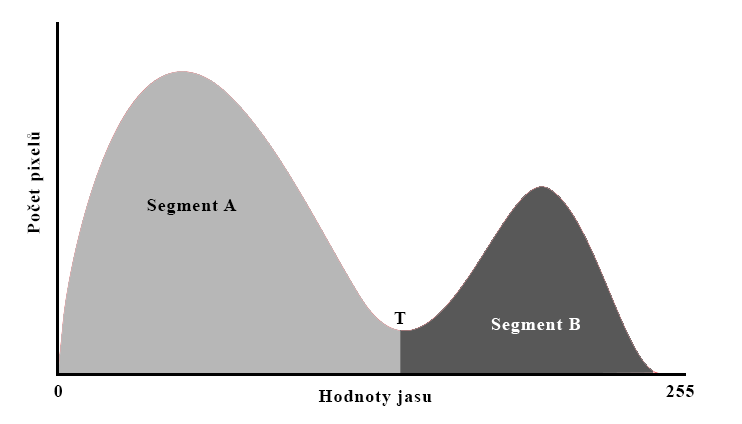
\includegraphics[height=6cm]{Figures/explanatory/histogram-auto-threshold.png}
	\caption{Nalezení ideálního prahu pomocí histogramu}
\end{figure}

\noindent
Druhou metodou je metoda založená na gradientu obrazové funkce. Gradient je první derivací pro obraz $f(x, y)$. Vysoká úroveň gradientu může být způsobena „rychlým“ přechodem mezi dvěma regiony. Tyto metody jsou především vhodné na obraz s minimálním množstvím šumu. Mezi běžně používané operátory patří například Sobelovy operátory, Laplaceův operátor, LoG a Cannyho operátor. Cannyho detekční algoritmus je považován za jeden z nejlepších, výhodou je nalezení skutečného maxima gradientu a následně pomocí dvojího prahování zajištuje detekci hran i v oblastech malého kontrastu. \cite{Canny}

\subsubsection{Hledání podobností}
Další skupinou segmentačních algoritmů jsou ty, hledající podobné oblasti v obraze. Výhodou oproti algoritmům založených na hledání hran je lepší odolnost vůči šumu. Algoritmy se opírají především o metodu rozšiřování regionu. Rozšiřování regionu probíhá v následujících čtyřech krocích. 

\begin{enumerate}
	\item Výběr počátečních pixelů (seedů)
	\item Nastavení kritéria pro podobnost (rozsah jasu nebo barvy)
	\item Procházení okolních pixelů a porovnání jejich hodnot proti nastavenému kritériu
	\item Zastavení procházení bodů, nesplňují-li žádné dostupné body dané kritérium.
\end{enumerate}
\noindent
V praktickém experimentu (popsaném dále) porovnáme různé způsoby měření vzdáleností, implementována je i právě tato metoda segmentace obrazu. Detailní popis Seed-Growing algoritmu je popsán dále v textu.
\newpage
\subsection{Grafová reprezentace obrazu}
Je metoda, kdy na obrazovou matici nahlížíme jako neorientovaný ohodnocený graf. Výtvoření grafu, je klíčovou záležitostí pro následné měření vzdáleností za pomocí geodetické metriky. Metody jako spektrální segmentace využívají spektrálního rozkladu Laplaceovy matice obrazového grafu. S metodou úzce souvisí metoda rezistivního měření vzdálenosti, které se budeme věnovat v dalších kapitolách textu.\par

\begin{figure}[H]
	\vspace*{+3.0mm}
	\centering
	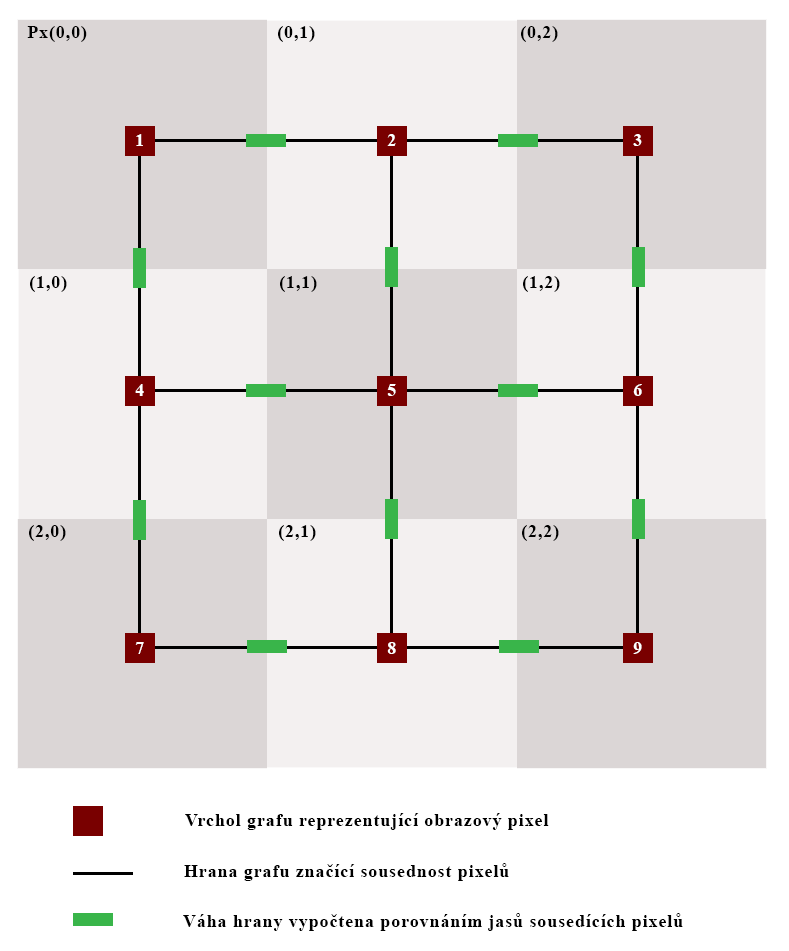
\includegraphics[height=13cm]{Figures/explanatory/imageAsGraph.png}
	\caption{Graf obrazové matice}
\end{figure}
\noindent
Na obrázku 6 vidíme šachovnicový podklad reprezentující jednotlivé pixely obrazu (pro přehlednost obraz má velikost pouze 3x3). Ke každému obrazovému pixelu je přiřazen jeden vrchol naležící výslednému grafu, sousedící pixely jsou propojeny ohodnocenou hranou. 
\newpage
\subsubsection{Implementace}
\begin{lstlisting}[label=src:Cpp,caption=Vytvoření obrazového grafu v jazyce C++]
void GenerateRGBVertexEdges(RGBVertex& vertex, const cv::Mat& img)
{

// Above

newX = vertex.GetX() + 0;

newY = vertex.GetY() - 1;

AddVertexNeighbour(newX, newY, m_imageGraph, vertex, img);

// Right

newX = vertex.GetX() + 1;

newY = vertex.GetY() + 0;

AddVertexNeighbour(newX, newY, m_imageGraph, vertex, img);

// Bellow

newX = vertex.GetX() + 0;

newY = vertex.GetY() + 1;

AddVertexNeighbour(newX, newY, m_imageGraph, vertex, img);

// Left

newX = vertex.GetX() - 1;

newY = vertex.GetY() + 0;

AddVertexNeighbour(newX, newY, m_imageGraph, vertex, img);

}
\end{lstlisting}

\subsubsection{Výpočet váhy}
Náš graf reprezentující obrazovou matici bude mít nepochybně tvar sítě (mesh). Váhy hran mezi jednotlivými vrcholy budou reprezentovat míru kontrastu mezi jednotlivými pixely v obraze. Zda budeme počítat i se sousedy na diagonálách, je již na ponecháno volnému rozhodnutí. Pro přehlednost diagramů a textu budeme v našem případě sousedy na diagonálách ignorovat. Obecně pro nás tedy platí, že každý uzel má 4 výstupní hrany vyjma pixelů na krajích obrazové matice. Každý pixel má informaci o svém jasu. V případě barevného obrazu můžeme jasovou složku vypočítat několika způsoby:\par

\begin{equation}
\vspace*{+3.0mm}
L = \frac{(R + G + B)}{3}
\end{equation}

\begin{equation}
\vspace*{+3.0mm}
L = (R * 0.21 + G * 0.72 + B * 0.07)
\end{equation}

\begin{equation}
\vspace*{+3.0mm}
L = \frac{\max(R, G, B) + \min(R, G, B)}{2}
\end{equation}

\noindent
Pro experiment v této práci jsme použili druhou metodu pro výpočet svítivosti (luminosity). Hodnota je důležitá, jelikož podle ní budeme vyčíslovat váhy hran v grafu. Váha grafu bude representovat jakousi cenu či odpor kterou musíme projít. Vyšší cena hrany proto znamená vysoký kontrast mezi danými pixely, které hrana spojuje. Hodnota hrany $0.0$ bude representovat absolutní kontrast kde jeden pixel je naprosto černý a druhý naprosto bílý. Hodnota hrany $1.0$ bude naopak reprezentovat, že oba pixely mají stejný jas.\par
Existuje řada způsobů, jak definovat váhu hrany, pro náš experiment jsem použil gausovu funkci. Gausián je definovaný obecným předpisem:

\begin{equation}
\vspace*{+3.0mm}
f(x) = ae^{- \frac{(z - \mu)^2}{2\sigma^2}}
\end{equation}
\noindent
Pro naše využití funkci upravíme na:
\begin{equation}
\vspace*{+3.0mm}
w_i, j = e^{- \frac{||b_i - b_j||^2}{2\sigma^2}}
\end{equation}
\noindent
$w_i, j$ je váha naší hrany mezi body $i$ a $j$.  $\sigma$ je zvolená konstanta. Volba správné konstanty není úplně přímočará záležitost a v mnoha textech je to považováno za otevřený problém. \cite{Zelnik} Mnoho výzkumníků nastavuje konstantu pouhým zkoušením. \cite{Jordan} Algoritmus spouštějí opakovaně a hledají nejlepší nastavení konstanty.

\begin{figure}[H]
	\vspace*{+3.0mm}
	\centering
	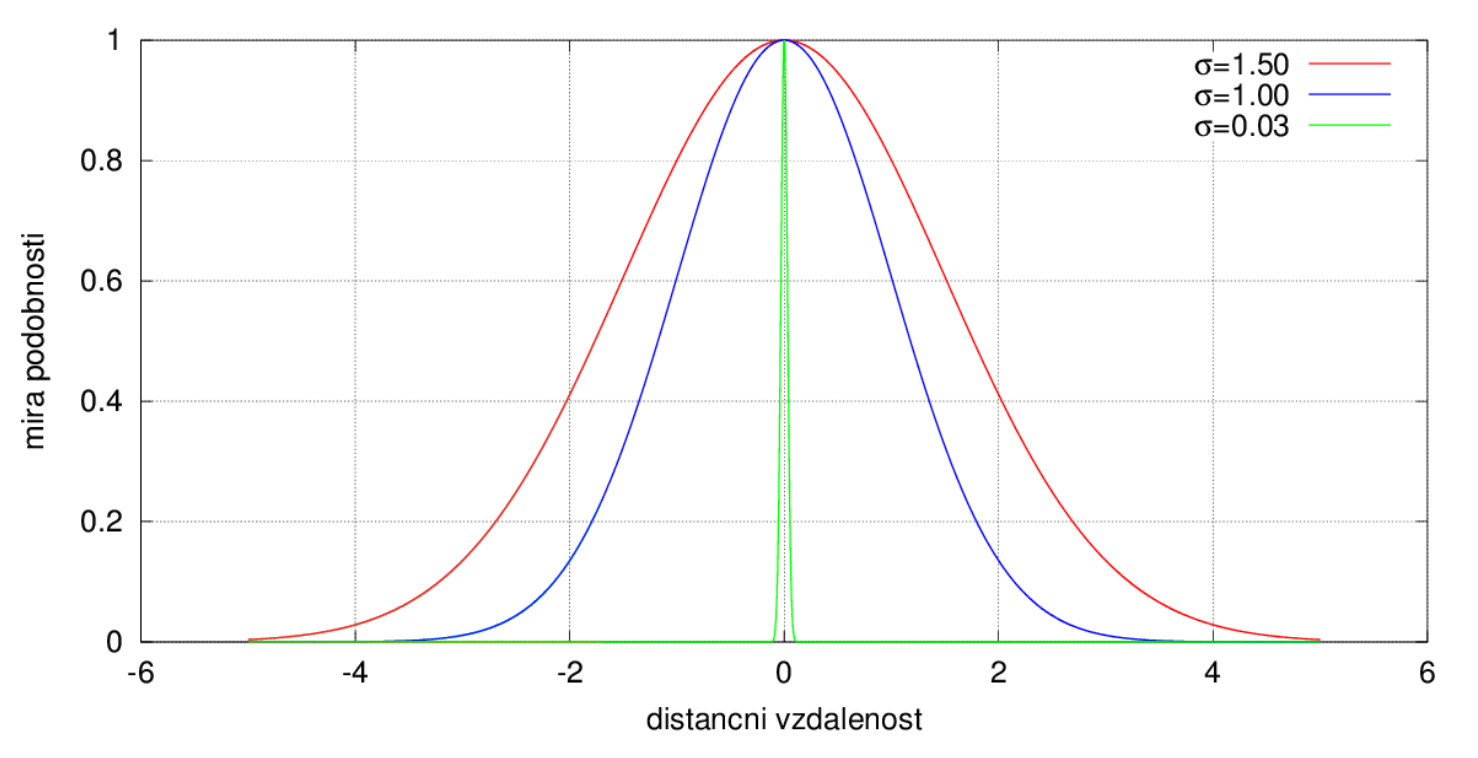
\includegraphics[height=8.5cm]{Figures/explanatory/gaussians.png}
	\caption{Gausova funkce s různými parametry $\sigma$ \cite{Pecha}}
\end{figure}
\noindent
Pro použití určení vah v našem obrazovém grafu je výhodné, aby se Gausián rostl resp. klesal co možná nejprudšeji. Dle statistického pravidla $3\sigma$ jsme pro náš experiment zvolili právě hodnotu kde $\sigma = 0.03$. Toto nám zajistí, že hodnoty vah u pixelů s podobným jasem budou velmi blízké $1$. Nadruhou stranu pixely s odlišným jasem budou mít podobnostní váhu ryhle blížící se $0$ u absolutně odlišných jasových hodnot ($0$ a $255$ - černá a bílá) .

\subsubsection{Implementace}
\begin{lstlisting}[label=src:Cpp,caption=Lambda funkce pro výpočet váhy grafu v C++]
auto calcWeight = [](RGBVertex& v1, RGBVertex& v2) 
{
	const double sigma = 0.03;

	double gaussian = exp(-((std::pow(
		std::fabs(((double)v1.GetLuminosity()) - 
			((double)v2.GetLuminosity())), 2)) / 2 
				* (std::pow(sigma, 2))));

return gaussian;

};
\end{lstlisting}

\subsection{Maticová reprezentace}
V této kapitole si popíšeme jak sestavit tzv. Laplaceovu matici. Jedná se o jeden ze základních prvků teorie grafů. V různých úlohách lze nalést různé definice, které jsou přizpůsobeny právě daným probémům. Pro naše účely (tedy využití v obrazové segmentaci) se budeme snažit definovat Laplaceovu matici tak aby co nejlépe popsala obrazový graf a jeho komponenty. Laplaceova matice existuje v normalizované a nenormalizované podobě, v tomto textu se ovšem zaměříme na její nenormalizovaný tvar. Laplaceovu matici $L$ definujeme jako rozdíl matice vrcholových stupňů $D$ a matice sousedností $A$. \cite{Dostal} \par

\begin{equation}
\vspace*{+3.0mm}
L = D - A
\end{equation}

\subsubsection{Matice stupňů vrcholů}
Anglicky nazývaná Degree matrix. V rovnici č. 5 ji značíme velkým písmenem $D$. Matice je velkosti $n \times n$ , kde $n$ je počet vrcholů v grafu. Matice je poměrně řídká a data se nacházejí pouze na diagonále. Daty matice jsou počty hran u každého vrcholu grafu. Na obrázku č. 8 máme graf $G$ a vytvořenou matici $D$ (rovnice 12).

\begin{figure}[H]
	\vspace*{+3.0mm}
	\centering
	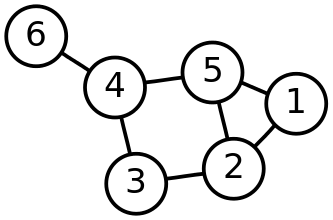
\includegraphics[height=4cm]{Figures/explanatory/laplacianGraph.png}
	\caption{Graf G}
\end{figure}

\begin{equation}
\vspace*{+3.0mm}
D = \begin{bmatrix} 
2 & 0 & 0 & 0 & 0 & 0 \\
0 & 3 & 0 & 0 & 0 & 0 \\
0 & 0 & 2 & 0 & 0 & 0 \\
0 & 0 & 0 & 3 & 0 & 0 \\
0 & 0 & 0 & 0 & 3 & 0 \\
0 & 0 & 0 & 0 & 0 & 1
\end{bmatrix}
\end{equation}

\subsubsection{Matice sousednosti}
Anglicky Adjacency matrix. Je matice popisující sousednost mezi vrcholy. Hodnoty matice jsou binární. Matice je taktéž velkosti $n \times n$, kde $n$ je počet vrcholů v grafu. Hodnota 1 udává, že mezi dvocicí vrcholů $m$ a $n$ existuje hrana, a naopak hodnota 0 reprezentuje fakt, že vrcholy spojené nejsou. Níže, je sestrojená matice sousednosti $A$ ke grafu G.

\begin{equation}
\vspace*{+3.0mm}
A = \begin{bmatrix} 
0 & 1 & 0 & 0 & 1 & 0 \\
1 & 0 & 1 & 0 & 1& 0 \\
0 & 1 & 0 & 1 & 0 & 0 \\
0 & 0 & 1 & 0 & 1& 1 \\
1 & 1 & 0 & 1& 0 & 0 \\
0 & 0 & 0 & 1 & 0 & 0
\end{bmatrix}
\end{equation}

\subsubsection{Laplaceova matice}
Samotné sestrojení Laplaceovy matice je více méně přímočarý postup. Podle rovnice č. 11 se jedná o rozdíl matice vrcholových stupňů a matice sousednosti. K ukázce využijeme graf G z obrázku 8 a k němu sestrojené matice $D$ a $A$. \cite{Dostal} Vztah č. 11 můžeme tedy přepsat na:

\begin{equation}
\vspace*{+3.0mm}
L = \begin{bmatrix} 
2 & 0 & 0 & 0 & 0 & 0 \\
0 & 3 & 0 & 0 & 0 & 0 \\
0 & 0 & 2 & 0 & 0 & 0 \\
0 & 0 & 0 & 3 & 0 & 0 \\
0 & 0 & 0 & 0 & 3 & 0 \\
0 & 0 & 0 & 0 & 0 & 1
\end{bmatrix} 
-
\begin{bmatrix} 
0 & 1 & 0 & 0 & 1 & 0 \\
1 & 0 & 1 & 0 & 1& 0 \\
0 & 1 & 0 & 1 & 0 & 0 \\
0 & 0 & 1 & 0 & 1& 1 \\
1 & 1 & 0 & 1& 0 & 0 \\
0 & 0 & 0 & 1 & 0 & 0
\end{bmatrix}
=
\begin{bmatrix} 
2 & -1 & 0 & 0 & -1 & 0 \\
-1 & 3 & -1 & 0 & -1 & 0 \\
0 & -1 & 2 & -1 & 0 & 0 \\
0 & 0 & -1 & 3 & -1 & -1 \\
-1 & -1 & 0 & -1 & 3 & 0 \\
0 & 0 & 0 & -1 & 0 & 1
\end{bmatrix}
\end{equation}

\noindent
Asi nikoho nepřekvapí, že Laplaceova matice je symetrická (vzhledem k faktu, že jak $D$ tak $A$ jsou taktéž symetrické). Při promyšlení jak vlastně matice vznikla je zřejmé, že determinant této matice je roven 0.

\begin{equation}
\vspace*{+3.0mm}
det(L) = 0
\end{equation}

\noindent
To způsobuje, že matice je tzv. singulární, a nelze tedy bežnými metodami nalézt její inverzní matici. Problém singulárnosti Laplaceovy matice prozkoumáme dále při výpočtu rezistivní vzdálenosti. 

\section{Měření vzdáleností}
V této kapitole si podrobně rozebereme možné techniky pro měření vzdáleností a jejich význam v algoritmech pro segmentaci obrazu. Pro mnohé nebude asi překvapením, že pro většinu segmentačních úloh je pro porovnávání pixelů použita právě vzdálenost přímky tedy vzdálenost euklidovská, a to i přes své podstatné nedostatky. Chyby mohou nastat právě při detekci oblastí, které plynule mění svůj jas či barvu (například horizont oblohy). Tento problém například řeší měření pomocí geodetické, případně rezistivní vzdálenosti.


\subsection{Euklidovská vzdálenost}
Euklidovská vzdálenost popisuje ''běžnou'' vzdálenost mezi dvěma body v euklidovském prostoru. Definováním této vzdálenosti se z euklidovského prostoru stane metrický prostor. Pro výpočet euklidovské vzdálenosti se využívá rovnice Pythagorovy věty:

\begin{equation}
\vspace*{+3.0mm}
p = (p_1, p_2, .... p_n), q = (q_1, q_2, .... q_n)
\end{equation}

\begin{equation}
\vspace*{+3.0mm}
d(p,q) = \sqrt{(p_1 - q_1)^2 + (p_2 - q_2)^2 + ... + (p_n - q_n)^2} = \sqrt{\sum_{i = 0}^{n} (p_i - q_i)^2 }
\end{equation}

\noindent
V našem případě vektory $p$ a $q$ reprezentují dva porovnávané obrazové pixely. Složky těchto vektorů odpovídají jednotlivým obrazovým kanálům. U klasického černobílého obrazu máme kanál pouze jeden, vektory budou mít pouze jednu složku, euklidovská vzdálenost je v takovémto případě rovná absolutní hodnotě rozdílu jasů porovnávaných pixelů. Pro tříkanálový obraz má vektor hodnoty tři.

\begin{figure}[H]
	\vspace*{+3.0mm}
	\centering
	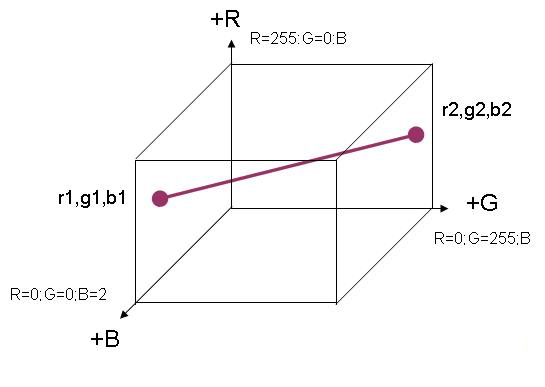
\includegraphics[height=6cm]{Figures/explanatory/euclideanDistance3d.jpg}
	\caption{Vizualizace EV pro RGB vektory}
\end{figure}
\noindent
Je samozřejmě možné, aby obraz měl více než 3 obrazové kanály. Další kanály mohou držet další informace jako například alfa-kanál (průhlednost) případně hloubkovou informaci (vzdálenost pixelu od kamery v době expozice snímku).  Do vektorů $p$ a $q$ lze samozřejmě přiřadit i další hodnoty než jednotlivé kanály obrazu. A to například hodnoty dopočítané ze sousedních pixelů jako průměr okolí, případně směrodatná odchylka. 

\subsubsection{Výhody}
Mezi asi největší výhodu je její přímočarý výpočet. Rovnice je jednoduše implementovatelná a snadná na pochopení. Současně se jedná i o velice rychlou metodu nevyžadující rozsáhlé procházení obrazu. V případech kdy máme obraz s jasně definovanými plochami bez jemných přechodů může metoda pro segmentaci nabízet velmi dobré výsledky.\par

\begin{figure}[H]
	\centering	
	\subfloat[Originál]{{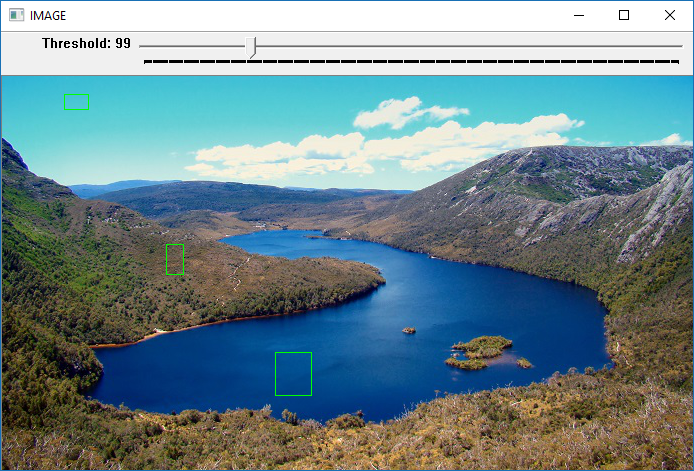
\includegraphics[width=7.5cm]{Figures/results/euclidean/img1/original.png} }}
	\subfloat[Segment oblohy]{{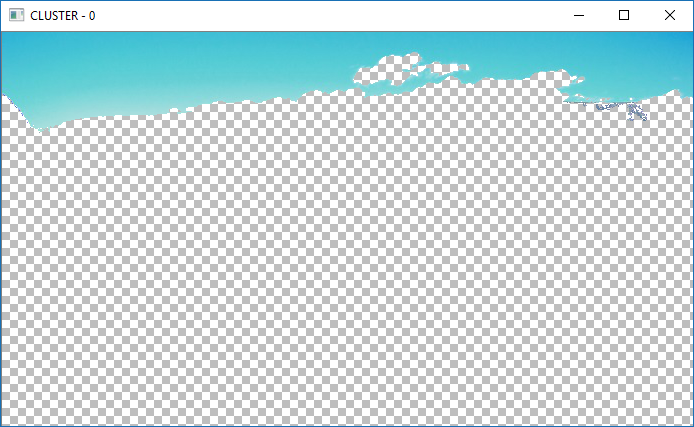
\includegraphics[width=7.5cm]{Figures/results/euclidean/img1/cluster0.png} }}
	\qquad
	\subfloat[Segment jezera]{{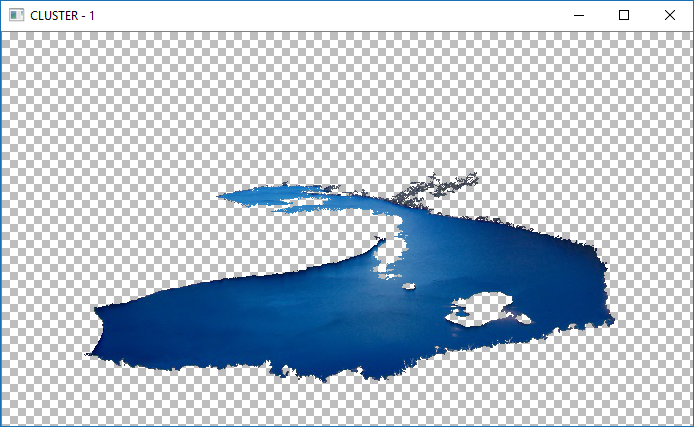
\includegraphics[width=7.5cm]{Figures/results/euclidean/img1/cluster1.png} }}
	\subfloat[Segment terénu]{{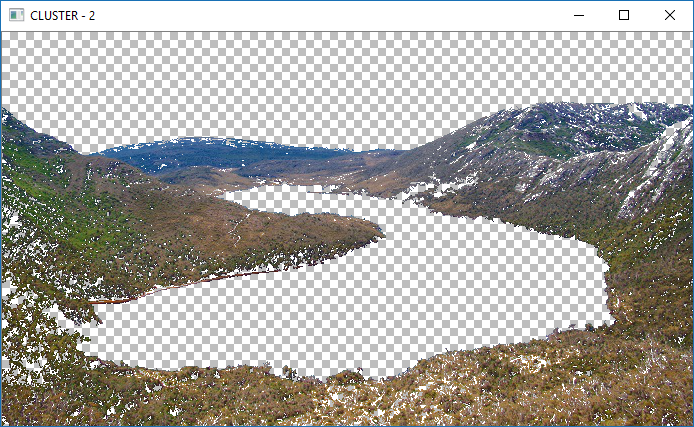
\includegraphics[width=7.5cm]{Figures/results/euclidean/img1/cluster2.png} }}
	\caption{Segmentace pomocí EV s použitím Seed-Growing algoritmu}
\end{figure}
\noindent
Ze skupiny obrázků 10, lze vidět segmentaci provedenou za pomocí euklidovské vzdálenosti. Viditelné jsou i nedostatky, kterýma segmentace pomocí euklidovské vzdálenosti trpí. Další ukázky se nacházení na konci textu v sekci přílohy.

\subsubsection{Nevýhody}
Nevýhod při použití euklidovské vzdálenosti v segmentaci obrazu je celá řada. Nicméně zda-li se daná nevýhody projeví, závisí na sofistikaci daného segmentačního algoritmu.
\begin{figure}[H]
	\vspace*{+3.0mm}
	\centering
	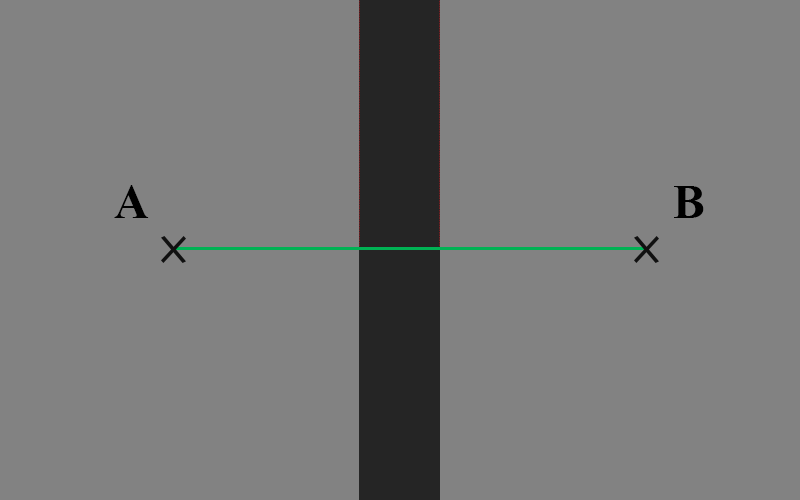
\includegraphics[height=5cm]{Figures/explanatory/euclideanMetric.png}
	\caption{Ignorování hrany euklidovskou vzdáleností}
\end{figure}
\subsubsection{Najivní přístup k segmentaci}
Najivním přístupem k segmentaci obrazu se dá nazvat postup jakkoliv ignorující spojité oblasti v obraze. U takovéhoto algoritmu máme definován počáteční seed (reprezentující hodnota shluku). Nýní procházíme všechny body v obraze a měříme euklidovskou vzdálenost vůči seed pixelu. Výsledek takovéto segmentace je zcela intuitivní, algoritmus zahrne do shluku všechny body v obraze s podobným jasem, či barvou (dle vektoru hodnot reprezentující obrazový pixel), které vyhovují definovanému prahu.

\begin{figure}[H]
	\centering	
	\subfloat[Originál]{{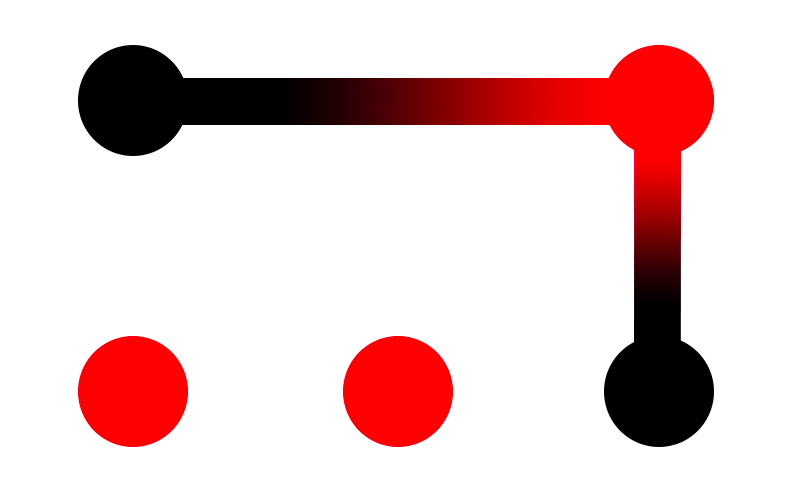
\includegraphics[height=4cm]{Figures/explanatory/proofOfConcept.png} }}
	\subfloat[Nalezené segmenty]{{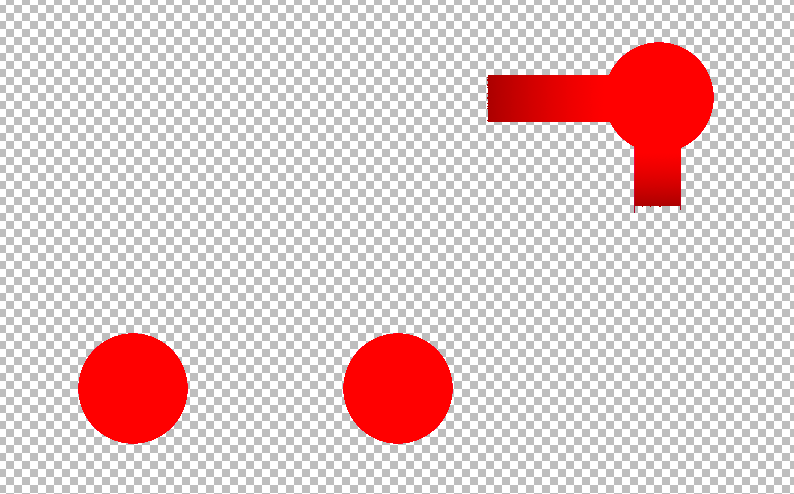
\includegraphics[height=4cm]{Figures/explanatory/ev-naive.png} }}
	\caption{Najivní segmentace pomocí EV}
\end{figure}

\subsubsection{Segmentace Seed-Growing algoritmem}
Způsobem jak ''vybruslit'' z velmi špatných výsledků dosažených najivní segmentací, je použití sofistikovanějšího algoritmu. Seed-Growing algoritmus neprochází slepě všechny obrazové pixely. Naopak využije seed pixelu jakožto počátečního bodu pro následné rozrůstání všemi směry. Algoritmus rekurzivně navštěvuje všechny sousedy daných bodů. Ve chvíli, kdy narazí na pixel, jehož naměřená EV větší než definovaný práh, program již dál tímto směrem nepokračuje a zkouší pixel jiný. To provádí do chvíle kdy jsou takovéto pixely k dispozici. \par

\begin{lstlisting}[label=src:Cpp,caption=Seed-Grow algoritmus,aboveskip=3em]
for (size_t i = 0; i < m_clusters[seed.GetCluster()].size(); i++)

{

	for (auto edge : m_clusters[seed.GetCluster()].at(i)->GetEdges())

	{

		// Jump over non-existing neighbours
		if (edge == nullptr)

			continue;

		
		RGBVertex tempVertex = *(edge->GetNeighbour());

		double tempDistance = GetEuclideanDistance(seed, tempVertex);

		
		if (tempDistance < m_threshold && tempVertex.GetCluster() == -1)

		{

			edge->GetNeighbour()->SetCluster(seed.GetCluster());

			m_clusters[seed.GetCluster()].push_back(edge->GetNeighbour());

		}

	}
}

\end{lstlisting}
Touto metodou lze nepochybě dosáhnou velice uspokojivých výsledků (skupina obrázků 10). Nicméně bohužel ani tato metoda není neprůstřelná pro všechny případy. \par 
Hlavním problémem oblasti s plynulým přechodem. U těchto oblasti v jistou chvíli dojde algoritmus k bodu, kde pixely již nevyhovují prahové hodnotě a oblast se "zařízne". Člověk samozřejmě vidí, že oblast pokračuje dále, pro řešení této problematiky je potřeba elegantnější řešení, které bere v potaz hodnotu sousedních pixelů, a cestu po které se algoritmus k danému pixelu dostal. Takovéto metody popisují další způsoby měření vzdáleností, jako je například vzdálenost geodetická nebo rezistivní. \par

\begin{figure}[H]
	\centering	
	\subfloat[Originál]{{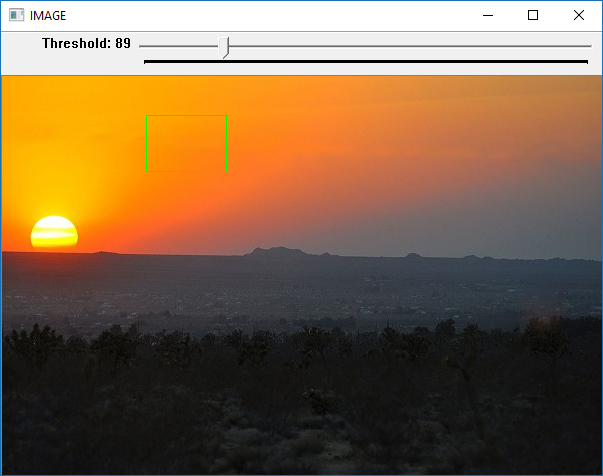
\includegraphics[width=10cm]{Figures/results/euclidean/img3/original.png} }}
	\qquad
	\subfloat[Segment oblohy]{{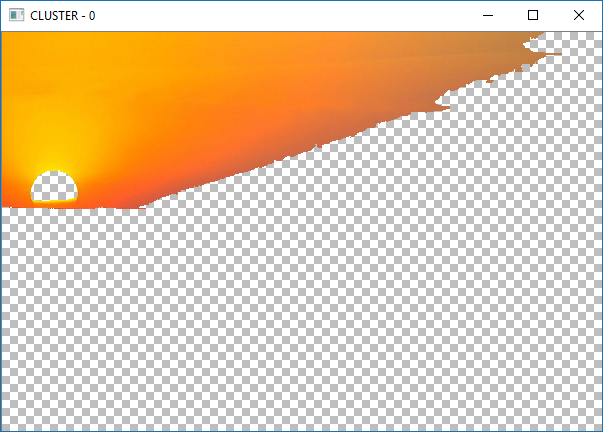
\includegraphics[width=10cm]{Figures/results/euclidean/img3/cluster0.png} }}
	\caption{Problém EV s jemnými přechody}
\end{figure}

\subsection{Geodetická vzdálenost}
Je obecně definována jako nejkratší vzdálenost mezi dvěma vrcholy v grafu. Větší smysl samozřejmě dává hledat nejkratší cestu v grafu ohodnoceném. Abychom tuto metodu měření mohli použít v našem obraze musíme vygenerovat obrazový graf reprezentující obrazovou matici. Postup toho procesu byl již vysvětlen v kapitole 3.5. \cite{Bouttier}
\begin{figure}[H]
	\vspace*{+3.0mm}
	\centering
	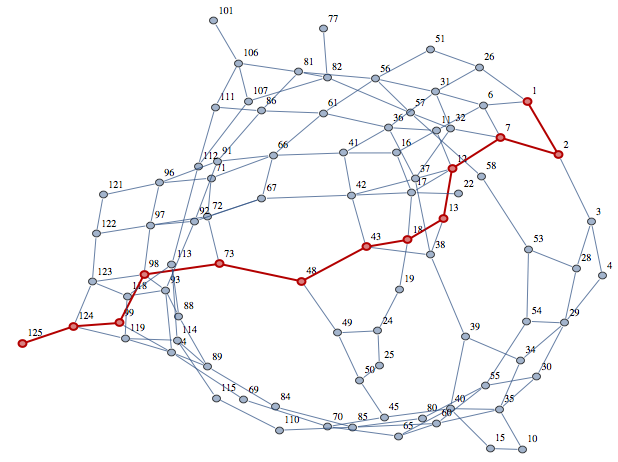
\includegraphics[height=9cm]{Figures/explanatory/geodesicDistanceBigGraph.png}
	\caption{Geodetická vzdálenost v obecném grafu}
\end{figure}


\subsubsection{Nalezení nejkratší cesty}
Tento problém je v informatice studován po mnoho let. Existuje celá řada algoritmů pro hledání nejkratší cesty v grafu, jako například Dijkstrův algoritmus nebo A-star (A*). Prvotně může nabízet řešení, použít algoritmus A*, jakožto efektivnější variantu Dijkstrova algoritmu. Nicméně pro náš konkrétní účel je výhodnější právě Dijkstrův algoritmus.\par
Hlavním rozdílem mezi algoritmy je fakt, že A* bere k úvahu i směr ve kterém se cíl nachází, například pomocí Euklidovské vzdálenosti. Algoritmus tedy neprochází všechny uzly, ale jen ty ležící ve směru cíle.  To by ovšem ve výsledku znamenalo, že bychom algoritmus museli pouštět vícekrát pro různé cíle, což by vedlo k opakovanému ohodnocování většiny bodů.\par
Z tohoto důvodu vhodnější použít právě Dijkstrův algoritmus a využít jeho nevýhodné (ale pro nás hodící se) vlastnosti, kterou je procházení všech uzlů. Dijkstrův algoritmus v jednom průchodu nalezne nejen nejkratší cestu do z počátečního bodu do cílového, ale současně všechny nejkratší cesty z počátečního bodu do bodů všech ostatních.\cite{Algfoor}\par

\subsubsection{Dijkstrův algoritmus}
Je nejrychlejší (v dnešní době známý) algoritmus pro hledání nejkratších cest z počátečního uzlu. Běh DA lze popsat  jako na zobecněné prohledávání grafu do šířky, kde se ''vyhledávací vlna'' šíří na základě vzdálenosti od zdroje (kde vzdálenost representuje váha hran). Algoritmus zpracovává pouze ty uzly, k nimž doposud nebyla nalezena nejkratší cesta.\par
DA si uchovává všechny vrcholy v seřazené prioritní frontě dle vzdálenosti od počátečního vrcholu – v prvním běhu má pouze zdroj vzdálenost 0, všechny ostatní uzly nekonečno. Algoritmus v každé své iteraci vybere z fronty vrchol s nejvyšší prioritou (resp. nejnižší vzdáleností od již zpracované části), následně je prvek zařazen mezi zpracované uzly. Poté projde všechny, jeho dosud nezpracované sousední uzly a přidá je do fronty nejsou-li tam již obsaženy. Následně je ověřena vzdálenost sousedních prvků od zdroje, zda-li nejsou blíže, než byli před zařazením právě vybraného uzlu mezi zpracované. To znamená, že pro všechny potomky ověřujeme:

\begin{equation}
\vspace*{+3.0mm}
w_i + e_{i, j} < w_j
\end{equation}
\noindent
Platí-li nerovnost, je danému potomkovi nastavena nová vzdálenost a označíme za jeho předka zpracovávaný uzel. Po průchodu přes všechny sousední vrcholy vybere algoritmus z fronty uzel s nejkratší cestou (nejvyšší prioritou) a iterace se opakuje.\par
Algoritmus se ukončí v okamžiku, kdy jsou všechny uzly zpracovány (prioritní fronta je prázdná). DA je použitelný jen v případě, obsahuje-li graf pouze nezáporně ohodnocené hrany – v případě záporných hran algoritmus není schopen garantovat, že při zpracování vrcholu byla již nalezena nejkratší možná cesta. \cite{Kolar}

\subsubsection{Složitost}
Složitost DA závisí na návrhu a implementaci prioritní fronty. V případě její implementace pomocí klasického sekvenčního seznamu je složitost algoritmu:

\begin{equation}
\vspace*{+3.0mm}
O(|U|^2)
\end{equation}
\noindent
Je-li fronta binární haldou pak:

\begin{equation}
\vspace*{+3.0mm}
O(|H|\log_2|U|)
\end{equation}

\newpage
\subsubsection{Implementace}
\begin{lstlisting}[label=src:Cpp,caption=Jádro dijskstrova algoritmu]
for (auto& e : start->GetEdges())

{
	// 	Preskoceni neexistujicich hran
	if (e == nullptr || e->GetNeighbour()->GetIsSeedDistanceFinal())

		continue;


	// Preskoceni sousedu s vyssim nez povolenym kontrastem
	if (e->GetResistance() > m_threshold)

		continue;


	double edgeWeight = e->GetResistance() + start->GetSeedDistance();

	double seedDistance = e->GetNeighbour()->GetSeedDistance();


	// Kontrola delky cesty
	if (edgeWeight <= seedDistance)

	{

		e->GetNeighbour()->SetSeedDistance(edgeWeight);

		m_knownVertices.push_back(e->GetNeighbour());

	}

}
\end{lstlisting}


\subsubsection{Způsob segmentace}
Při využití geodetické vzdálenosti je zapotřebí segmentační algoritmus upravit tak aby samotný Dijkstrův algoritmus rozhodoval o přiřazení pixelu do clusteru. Způsobů jak tohoto docílit je několik. Přínos geodetické vzdálenosti je především v tom, že zvládá rozpoznat i oblasti a proměnným jasem, mění-li se míra jasu pozvolna.\par
Dijkstrův algoritmus obdrží náš seed pixel jako počáteční bod a libovolný jiný pixel jako bod cílový. Připomeňme, že Dijkstrův algoritmus vždy projde všechny body v obraze a nalezne všechny nejkratší cesty z počátečního uzlu. Výhodou je právě inkrementální přístup k počítání vzdálenosti. Algoritmus postupně prochází jednotlivé hrany, které v případě malé jasové změny mají minimální hodnotu. Při nalezení hrany s hodnotou větší, než definovaný práh tuto hranu ignorujeme, a bod k ní připojený prozatím nepovažujeme za součást segmentu. Není ovšem vyloučeno, že daný bod bude přiřazen do segmentu z jiné cesty.\par

\begin{figure}[H]
	\centering	
	\subfloat[Originál]{{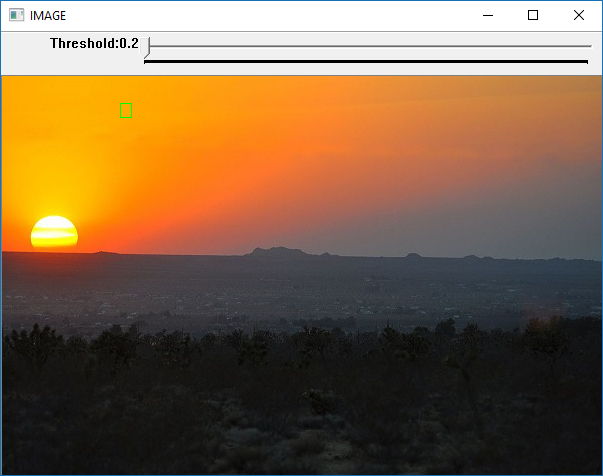
\includegraphics[height=6cm]{Figures/results/geodesic/img3/original.png} }}
	\subfloat[Segment oblohy]{{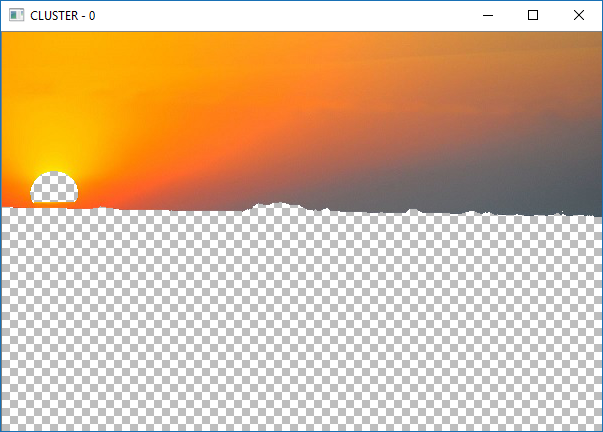
\includegraphics[height=6cm]{Figures/results/geodesic/img3/cluster0.png} }}
	\caption{Segmentace pomocí GV}
\end{figure}
\noindent
Na obrázku 15 můžeme vidět segment celého horizontu, algoritmus přesně dle teorie propojil oblasti s jemným přechodem a zastavil se na oblastech kde je změna v kontrastu razantní. Ukázka dalších obrázků experimentu bude součástí přílohy práce.\par

\subsubsection{Výhody}
Hlavní výhodou je právě schopnost detekování oblastí s proměnným jasem. Současně máme několik možností, jak nastavovat míru akceptovatelného přechodu (co považujeme za přechod a co už je součást jiné oblasti). První možností je aplikace prahu, který bude ignorovat hrany určité váhy. Současně můžeme modifikovat konstantu sigma u funkce Gausiánu při generování hran grafu.

\subsubsection{Nevýhody}
Poměrnou nevýhodou je relativně vysoká výpočetní složitost. Nejprve je zapotřebí vygenerovat obrazový graf a spočítat váhy mezi pixely. Následně samotný běh Dijkstrova algoritmu nad (v nejhorším případě) celým obrazem. Z hlediska kvality segmentace se objevují problémy další. Existuje-li v obraze pouze jediná cesta mírného kontrastu mezi dvěma oblastmi, algoritmus oblasti spojí skrz tuto cestu, problém je situace kdy cesta může být způsobená šumem jakéhokoliv původu (digitální či optická vada, neočekávaný objekt).

\begin{figure}[H]
	\vspace*{+3.0mm}
	\centering
	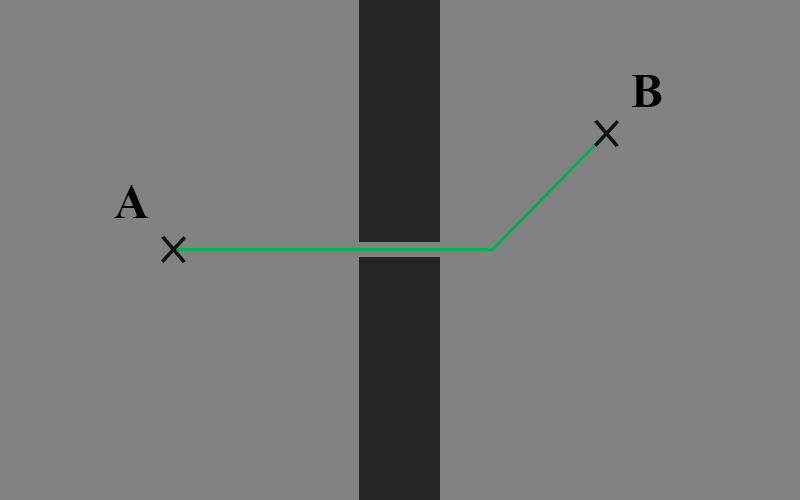
\includegraphics[height=5cm]{Figures/explanatory/geodesicMetric.png}
	\caption{Nalezení nekonečné tenké cesty}
\end{figure}

\subsection{Rezistivní vzdálenost}
Jedná se o metodu v mnoha směrech podobnou geodetické vzdálenosti. Stejně jako geodetická vzdálenost metoda pracuje nad grafem reprezentující obrazovou matici. Nicméně tam, kde geodetická vzdálenost bere vážně i jen jednu jedinou, libovolně tenkou cestu - rezistivní vzdálenost bere k úvahu cesty všechny. \cite{Klein}\par
Vzdálenost mezi dvěma body je tedy definována jakožto efektivní rezistivní vzdálenost společných bodů na pravidelné síti (našem grafu), kde každá hrana reprezentuje elektrický rezistor od oporu dle váhy hrany. Rezistor 1 Ohm reprezentuje maximální kontrast v obraze, rezistor 0 ohm representuje pixely stejného jasu. Hodnotu rezistoru získáme pomocí rovnice 10. Současně je důležité, že rovnice Gausiánu ve tvaru ve kterém je uvedena, vrací převácenou hodnotu odporu tedy vodivost. Zhlediska zjednodušení následného výpočtu, je výhodnější ukládat v obrazové matici právě vodivost. \par
Rezistivní vzdálenost přistupuje ke grafu jako k elektrickému obvodu, kde vzdálenost mezi dvěma body je definována jako proud procházející daným uzlem při připojení ideálního zdroje napětí mezi dvojici měřených bodů. Výpočet vychází z Laplaceovy matice obrazového grafu a Kirchhoffových zákonů.

\subsubsection{Kirchhoffovy zákony}
Jsou základním nástrojem teoretické elektrotechniky při návrhu elektrických obvodů. Byly definovány Gustavem Robertem Kirchhoffem v roce 1845. Dvojice zákonů popisuje zachování energie a elektrického náboje v uzavřeném okruhu. První Kirchhoffův zákon je definován jako:

\begin{definition}
	Algebraický součet proudů v uzlu je roven nule.
\end{definition}
\begin{equation}
\vspace*{+3.0mm}
\sum_{k = 1}^{k} (I_k) = 0 
\end{equation}

\noindent
Jinými slovy zákon definuje, že proud vstupující do uzlu obvodu, je roven proudu, který z uzlu vystupuje. Jedná se o reformulaci zákonu o zachováni energie. 

\noindent
Druhý Kirchhoffův zákon hovoří o úbytcích napětí na součástkách.
\begin{definition}
	Algebraický součet napětí ve smyčce je roven nule.
\end{definition}
\begin{equation}
\vspace*{+3.0mm}
\sum_{k = 1}^{k} (U_k) = 0 
\end{equation}

\noindent
Matematický aparát ve formě Kirchhoffových zákonů nám nyní umožňuje odvodit vzorec pro rezistivní vzdálenost. Máme-li vektor potenciálů $f$, který reprezentuje úrovně napětí na všech uzlech el. obvodu (respektive vrcholech obrazového grafu). Vektor $r$ obsahující hodnoty možných proudů přicházejících do a vycházejích ven z daného uzlu. S využitím prvního Kirchhoffova zákona, říkajícího že součet všech externích proudů je roven 0, dostaneme rovnici

\begin{equation}
\vspace*{+3.0mm}
Lf = r
\end{equation}
\noindent
kde $L$ je Laplaceova matice obsahující vodivosti. 

\subsubsection{Využití Laplaceovy matice}
Obecnou definici Laplaceovy matice jsme již probrali v kapitole 3. Nyní se zaměříme na její využití v segmentaci obrazu pomocí rezistivní vzdálenosti. Rovnice 24 zobrazuje Laplaceovu matici k jednoduchému $3 \times 3$ obrazu. Mějme definovat efektivní rezistivní vzdálenost mezi body $i$ a $j$. Pro tuto potřebu předpokládáme, že proud přitéká do obvodu bodem $i$ a následně dle 1. KZ stejný proud z bodu $j$ odtéká. Tento jev způsobí rozložení elektrických potenciálů v celém obvodu. Využitím Ohmova zákona můžeme odvodit, že efektivní rezistence mezi $i$ a $j$ je rovna $R_{i,j} = f_i - f_j$. Efektivní vodivost je definována jako převrácená hodnota rezistence $C_{i,j} = 1 / R_{i,j}$. Nyní se konečně dostaneme k roli Laplaceovy matice. \par
Nacházíme se ve stavu kdy máme rovnici 23, kterou potřebujeme řešit pro $f$. V běžném případě bychom definovali inverzní matici $L^{-1}$ a jí vynásobili vektor proudů $r$. Bohužel z definice Laplaceovy matice již víme, že matice je tzv. singulární. Co mimo jiné znamená, že determinant takovéto matice je roven 0. Iverze matice je definována jako násobení matice převrácenou hodnotou determinantu. Tu ovšem pro nulový determinant nelze nalést, jelikož bychom dostali zlomek s 0 ve jmenovateli. Pro převedení Laplaceovy matice na druhou stranu rovnice je zapotřebí vypočítat Moore-Penrosovu pseudoinverzi.
\begin{equation}
f = L^+ r
\end{equation}
\noindent
Kde $L^+$ je Moore-Penrosova pseudoinverze Laplaceovy matice, můžeme tedy odvodit vztah
\begin{equation}
R_{i,j} = (L^+_{i,i} - L^+_{i,j}) -  (L^+_{j,i} - L^+_{j,j}) = L^+_{i,i} - 2L^+_{i,j} + L^+_{j,j}
\end{equation}
\noindent
Hodnotami $L^+_{i,j}$ máme na mysli $i-tý$ řádek a $j-tý$ sloupec v matici $L^+$ (přípustná je i obrácená možnost jelikož $L^+$ je symetrická). Nejedná se tedy stejné souřadnice jako jsou hodnoty $x, y$ v obrazové matici. Z obrázku a 17 a rovnice 26 níže vidíme vztah mezi obrazovým grafem a Laplaceovou maticí. Dimenze Laplaceovy matice je rovna počtů bodů v samotném obraze. Lze tedy tvrdit, že počet prvků $L$ roste vůči počtu obrazových pixelů kvadraticky. Tento fakt působí nemalý problém pro reálnou implementaci rovnice 24. Výpočet pseudoinverze pro matici, která může bez problému obsahovat miliardy prvků (62,5 miliardy prvků pro obrázek $500\times500$px) je pro současný dostupný hardware velice zdlouhavý počin.
\begin{figure}[H]
	\vspace*{+3.0mm}
	\centering
	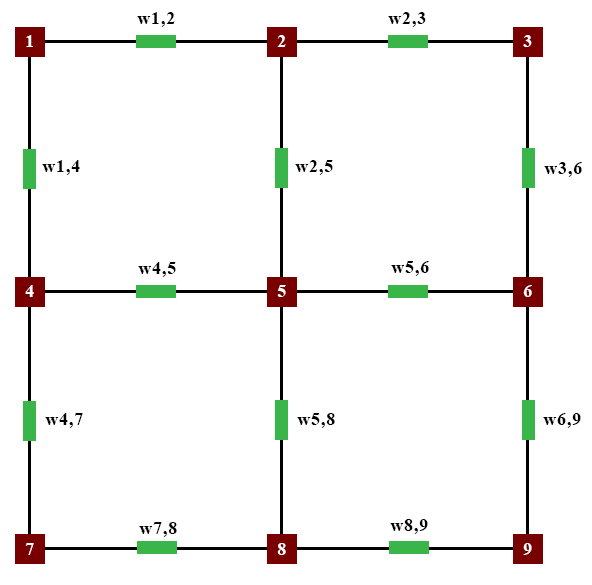
\includegraphics[height=4.5cm]{Figures/explanatory/resistanceGraph.png}
	\caption{Obrazový graf s rezistory}
\end{figure}

\begin{equation}
\vspace*{+3.0mm}
\resizebox{.9\hsize}{!}{$
L= \begin{bmatrix} 
	w_{1,2} + w_{1,4} & -w_{1,2}  & 0 & -w_{1,4} & 0 & 0 & 0 & 0 & 0 \\[1em]
	-w_{1,2} & w_{1,2} + w_{2,3} + w_{2,5} & -w_{2,3} & 0 &  -w_{2,5} & 0 & 0 & 0 & 0 \\[1em]
	0 & -w_{2,3} & w_{2,3} + w_{3,6} & 0 & 0 & -w_{3,6} & 0 & 0 & 0 \\[1em]
	-w_{1,4}  & 0 & 0 & w_{1,4} + w_{4,5} + w_{4,7} &  -w_{4,5} & 0 & -w_{4,7} & 0 & 0 \\[1em]
	0 & -w_{2,5} & 0 & -w_{4,5} & w_{2,5} + w_{4,5} + w_{5,6} + w_{5,8} &  -w_{5,6} & 0 & -w_{5,8} & 0 \\[1em]
	0 & 0 & -w_{3,6} & 0 & - w_{5,6} & w_{3,6} + w_{5,6} + w_{6,9} & 0 & 0 & -w_{6,9} \\[1em]
	0 & 0 & 0 & -w_{4,7} & 0 & 0 & w_{4,7} + w_{7,8} & -w_{7,8}  & 0 \\[1em]
	0 & 0 & 0 & 0 & -w_{5,8} & 0 & -w_{7,8} & w_{5,8} + w_{7,8} + w_{8,9}  & -w_{8,9} \\[1em]
	0 & 0 & 0 & 0 & 0 & -w_{6,9} & 0 & -w_{8,9} & w_{6,9} + w_{8,9}
\end{bmatrix}
$}
\end{equation}

\subsubsection{Implementace}
\begin{lstlisting}[label=src:Cpp,caption=Tvorba Laplaceovy matice v C++]
void ResistanceClustering::CalculateLaplacian()

{

	for (int v = 0; v < (int)m_image->GetImageGraph().size(); v++)

	{

		// Place sum of edges on diagonal;

		m_laplacian->at<float>(v, v) = SumEdges(m_image->GetImageGraph()[v]);
	
		// Place weights in laplacian

		for (auto& e : m_image->GetImageGraph()[v].GetEdges())

		{

			int laplacianIndex = (e->GetNeighbour()->GetY() *

			m_image->GetWidth() + e->GetNeighbour()->GetX());

			
			// Matrix is symetric therefor we swap the coordinates

			m_laplacian->at<float>(laplacianIndex, v) = -e->GetConductance();

			m_laplacian->at<float>(v, laplacianIndex) = -e->GetConductance();

		}

	}

}
\end{lstlisting}
\subsubsection{Řešení pomocí lineárních rovnic}
Vzhledem k rozměrům Laplaceovy matice u reálného obrazu, je provedení inverze v rozumném čase velice výkonově náročné. Alternativou je využití řešení lineárních rovnic. Postup vypadá zhruba takto. \par
Snažíme se o nalezení rezistivní vzdálenosti mezi uzly $i$ a $j$. Nastavíme tedy příslušné hodnoty vektoru potenciálů $f$ na pozicích $i$ a $j$ tak aby $f_i = 1$ a  $f_j = 0$. Tímto simulujeme připojení obvodu k ideálnímu zdroji napětí. Následně můžeme řešit rovnici 23, kde získáme vektor $r$. Nyní z matice $L$, vektorů $f$ a $r$ odebereme hodnoty na pozicích $i,j$. \par
V tuto chvíli matice L přestává být singulární a rovnice 23 se stává řešitelnou pro nalezení vektoru $f$ za pomocí klasických metod. Proudy procházející soustavou lze lehce určit za pomocí Ohmova zákona, jelikož již známe napětí i odpor v jednotlivých uzlech. Hledaná vodivost je rovna velikosti tohoto proudu.\cite{Gaura}

\subsubsection{Nevýhody a problémy}
Hlavní nevýhodou je zcela jistě zdlouhavý výpočet. Nutnost práce s velkou Laplaceovou maticí bývá v implementaci výzvou v několika rovinách. I přestože je matice $L$ řídká a prakticky plná nul, je manipulace s takovou maticí problematická. Jediným řešením je omezit velikost vstupních dat na nejmenší únosnou úroveň.\par
Další nevýhodou dle mého názoru je fakt, že výsledky segmentance nejsou nijak oslňující. Ve své dizertační práci Jan Gaura popisuje rezistivní vzdálenost jako obecně nevhodnou pro smysl obrazové segmentace. V textu je popisován problém kdy vstupní a výstupní bod pro měření je umístěn do homogenní oblasti, kde již existuje maximální možná vodivost, toto se v elektrickém obvodu nazývá zkratem. Druhou opačnou situací je problém, kdy dva měřené body jsou umístěny do dvou různých oblastí stejné plochy, které nespojuje žádná cesta.  \cite{Gaura}

\begin{figure}[H]
	\centering	
	\subfloat[Situace 1]{{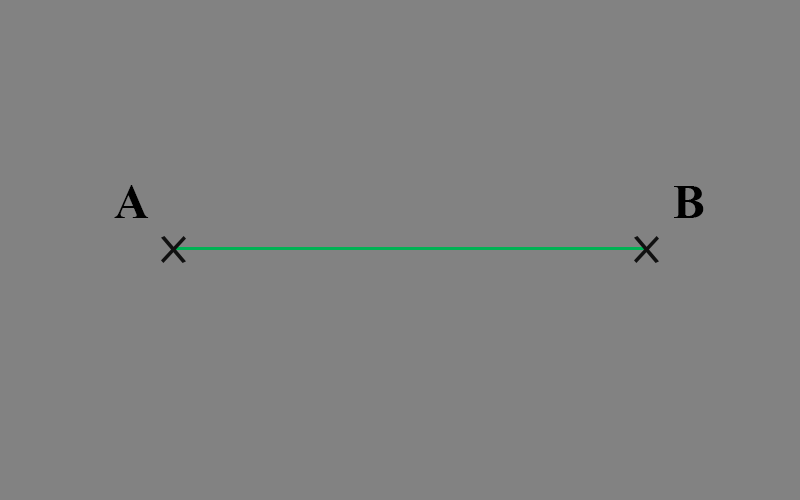
\includegraphics[height=4cm]{Figures/explanatory/resistanceIssue1.png} }}
	\subfloat[Situace 2]{{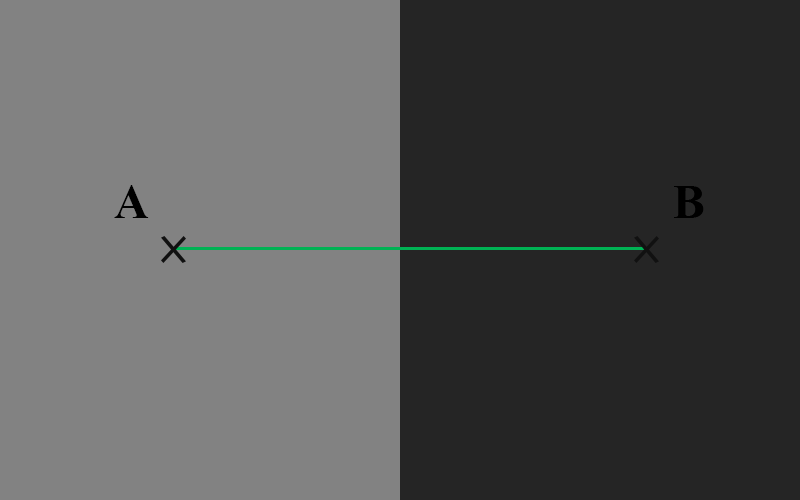
\includegraphics[height=4cm]{Figures/explanatory/resistanceIssue2.png} }}
	\caption{Problémy RV}
\end{figure}

\section{Implementace experimentu}
Nyní již máme teoretický základ toho jak jednotlivé metody měření vzdáleností fungují. Součástí této práce je i experimentální prozkoumání těchto metod a vyvození závěrů, které metody poskytují nejuspokojivější výsledky ve specifických situacích.


\subsection{Použité technologie}
Pro implementaci experimentální aplikace jsem dle zadání zvolil jazyk C++. Pří vývoji aplikace jsem kladl důraz na multiplatformní kompilvatelnost. Záměrně jsem se tedy vyhýbal použití veškerých plaformě závislých knihoven a rozhraní (jako například Windows API, Posix, X11). Aplikace využivá prvky standardu C++ 11, jako jsou lambda funkce a auto for cykly. Veškeré použité funkce a prvky jsou použity ze standardní STD knihovny, pro zaručení multiplaformního běhu a kompilace. Pro práci s obrazem jsem využil OpenCV knihovnu verze 3.2.0

\subsubsection{OpenCV}
Knihovna OpenCV neboli Open Computer Vision poskytuje sadu rozhraní, datových typů a algoritmů pro běžnou práci s obrazem. Knihovna taktéž garantuje multiplatformní kompilovatelnost. Výhodou je především vyřešené zobrazení uživatelského rozhraní na všech platformách. I když je zapotřebí dodat, že možnosti kontrolních prvků v OpenCV jsou velmi omezené, nicméně pro naše využití dostačující. \par

\begin{figure}[H]
	\vspace*{+3.0mm}
	\centering
	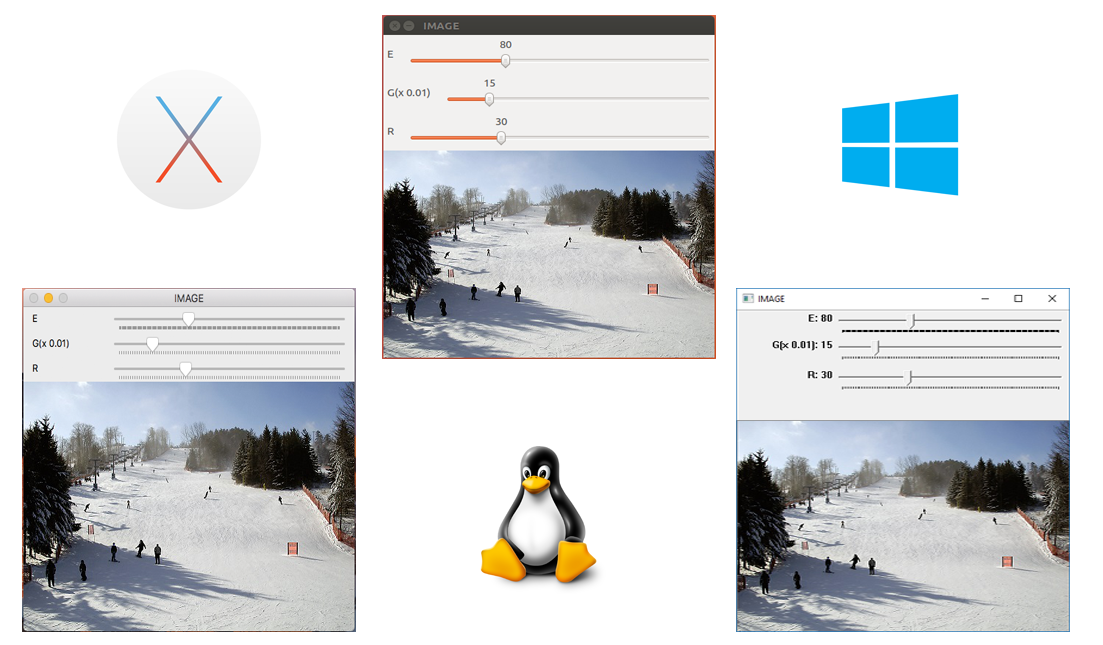
\includegraphics[height=7.3cm]{Figures/explanatory/multiplatform.png}
	\caption{Multiplatformní běh aplikace}
\end{figure}
\noindent
Poznámka: Na platformě OS X je bohužel nefunkční zobrazení hodnot vybraných posůvníkem, problém řeším duplicitním zobrazením vybraných hodnot v konzoli.\par

\noindent
Pro implementaci jsem využil v době psaní tohoto textu poslední verzi knihovny 3.2.0. Aplikace je s knihovnou linkovaná dynamicky. Součástí aplikace jsou již i zkompilované verze knihovny pro Windows platformu. Pro Unixové platformy je potřebná  opětovná rekompilace aplikace s knihovnami OpenCV korektně nainstalovanými v systému. Pro rekompilaci Windows verze aplikace je potřeba využít stejného kompilátoru jakým byly vytvořeny .lib a .dll soubory. Detaily o verzích jsou obsaženy v technické specifikaci aplikace, která je součástí přílohy této práce.

\subsection{Struktura}
I přes relativně jednoduchou vnitřní strukturu programu, jsem se snažil držet všech zásad objektově orientovaného programování. Jednotlivé shlukovací algoritmy jsou implementovány jako polymorfní dědičnost. Kde abstraktní třída SegmentationAlg reprezentuje všechny algoritmy, jejich vlastní třídy tuto třídu rozšiřují.
\begin{figure}[H]
	\vspace*{+3.0mm}
	\centering
	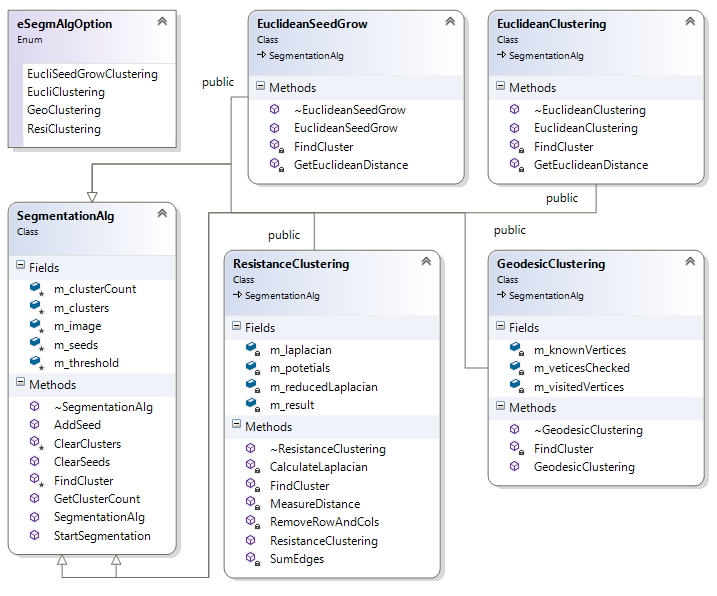
\includegraphics[width=14cm]{Figures/explanatory/classDiagramPoly.png}
	\caption{Třídní diagram shlukovacích algoritmů}
\end{figure}

\noindent
Zbylé třídy aplikace se zabývají kontrolou běhu aplikace a grafovou reprezentací obrazové matice. Nezbytnou součástí jsou i funkce počítající váhy v grafu pomocí gaussovy funkce. 

\subsection{Práce s aplikací}
Pro běh aplikace je potřeba nahrání obrázku, zadáním názvu obrázku jako parametru při spouštění aplikace. Aplikace pracuje pouze s jedním obrázkem, a to z důvodu, že v tuto chvíli standartní knihovny C++ neumožňují procházení složek jinak, než s využitím platformě závislých prvků. File system knihovna bude součástí C++ až od standardu C++ 17. \par
\begin{figure}[H]
	\centering	
	\subfloat[Konzole]{{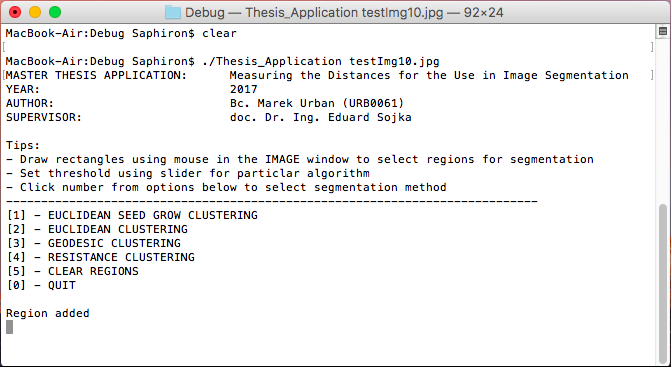
\includegraphics[height=6cm]{Figures/explanatory/console.png} }}
	\subfloat[Okno OpenCV]{{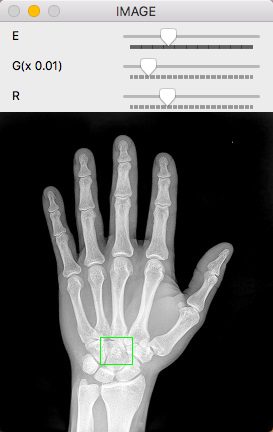
\includegraphics[height=6cm]{Figures/explanatory/app-region.png} }}
	\caption{Uživatelské rozhraní aplikace}
\end{figure}
\noindent
Uživatelské rozhraní, které knihovna OpenCV nabízí je velmi omezené. Pravdou je, že OpenCV umožňuje relativně snadnou integraci s například Qt frameworkem, nicméně aplikace slouží pouze jako experimentální podklad k teoretickému materiálu této práce. Komfortní uživatelské rozhraní tedy není prioritou. \par
Při spuštění aplikace a po korektním načtení obrázku se v konzolovém výstupu zobrazí menu s ovládacími prvky. Současně se otevře IMAGE okno s načteným obrázkem. Okno umožňuje nastavovat práhy pro euklidovskou, geodetickou a rezistivní metriku. Současně lze do okna zakreslit myší region určený k segmentaci. Z vybraného regionu se vypočte medián, který následně slouží jako seed (počáteční pixel) pro segmentaci regionu. Aplikace umožňuje vybrat libovolný počet regionů. Pro spuštění segmentace je důležité nad IMAGE oknem zmáčknout jednu z kláves popsaných v menu. Aplikace provede segmentaci dle zvoleného algoritmu a zobrazí jednotlivé segmenty v separátních oknech. Segmentaci nad stejnými regiony s jiným prahem lze provést snadno pouze změnou prahu na příslušném posuvníku a opětovném zmáčknutí dané klávesy. Pro opravu regionu je potřeba regiony promazat příslušnou klávesou a zakreslit nové regiony znovu.\par
Důležité je poznamenat, že záleží na pořadí v jakém byly dané regiony zadány. Z definice shlukování víme, že jeden bod se nemůže nacházet ve více segmentech, tedy pokud již bod byl přiřazen jinému segmentu, je automaticky ignorován při následné segmentaci s jiným seed pixelem. 

\section{Výsledky experimentu}
V předchozích kapitolách jsme si, jak popsali teoreticky princip jednotlivých metod měření vzdáleností, tak jsme si dané metody naimplementovali pomocí C++ aplikace. Ve čtvté kapitole jsme si ukázali výhody a nevýhody jednotlivých přístupů k měření vzdáleností. Nyní nahlédneme na výsledky dosažené naší experimentální aplikací a popíšeme si v čem jsou jednotlivé silné a slabé stránky jednotlivých způsobů měření vzdáleností.

\subsection{Euklidovská vzdálenost}
V této sekci se podíváme na naměřené výsledky pomocí euklidovské vzdálenost na bežných obrázcích různého charakteru. V některých situacích byla použita najivní segmentace v jiných segmentace pomocí růstu regionů (dle popisu).
\begin{figure}[H]
	\centering	
	\subfloat[Originál]{{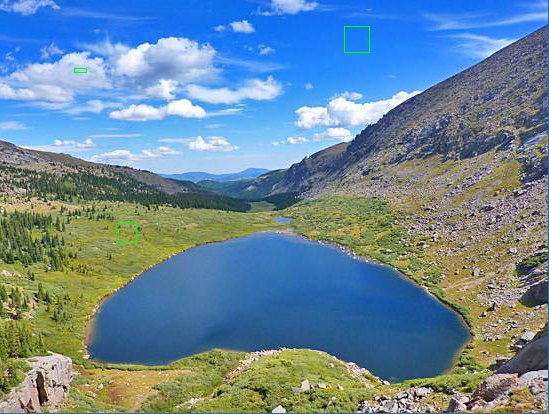
\includegraphics[width=7cm]{Figures/results/euclidean/img6/original.png} }}
	\subfloat[Segment 1]{{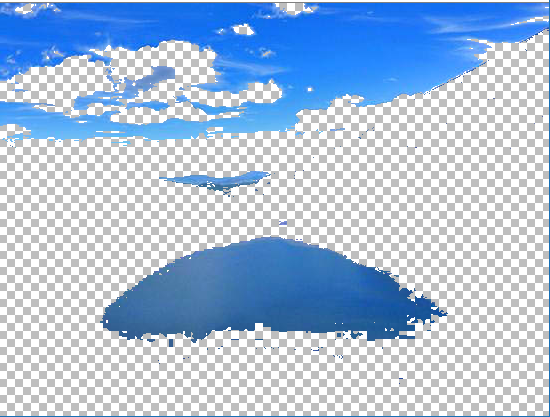
\includegraphics[width=7cm]{Figures/results/euclidean/img6/cluster1.png} }}
	\qquad
	\subfloat[Segment 2]{{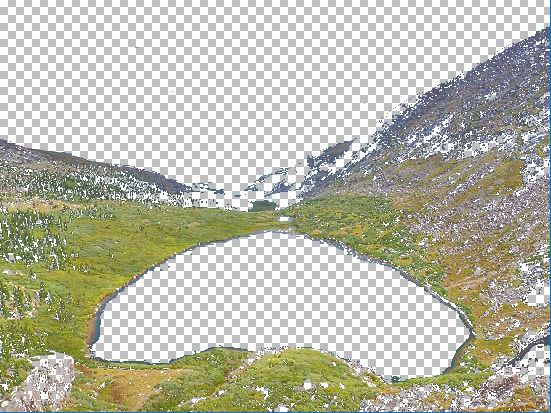
\includegraphics[width=7cm]{Figures/results/euclidean/img6/cluster2.png} }}
	\subfloat[Segment 3]{{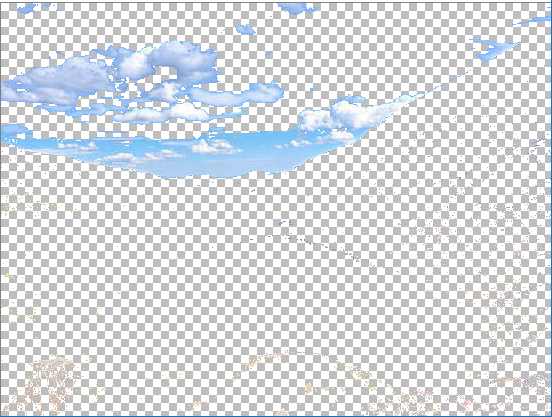
\includegraphics[width=7cm]{Figures/results/euclidean/img6/cluster3.png} }}
	\caption{Ukázka najivní segmentace}
\end{figure}
\newpage
\noindent
Z ukázky segmentace na obrázku 22 můžeme vidět problém euklidovské vzdálenosti. I přestože byla zadána segmentace oblohy  algoritmus nalezl i jezero vzhledem ke stejné barvě, zde tedy byla euklidovská vzdálenost nízká i přestože se jedná o úplně jinou oblast v jiné části obrazu. Problém částečně řeší použití lepšího segmentačního algoritmu.
\begin{figure}[H]
	\centering	
	\subfloat[Originál]{{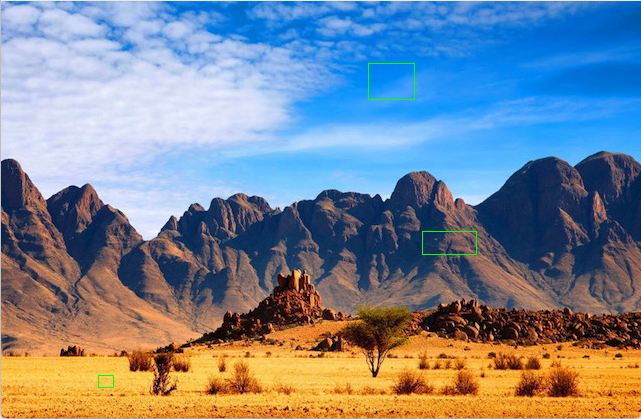
\includegraphics[width=7cm]{Figures/results/euclidean/img4/original.png} }}
	\subfloat[Segment 1]{{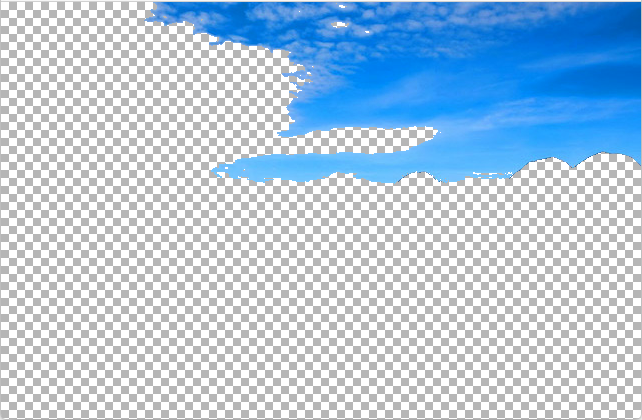
\includegraphics[width=7cm]{Figures/results/euclidean/img4/cluster1.png} }}
		\qquad
	\subfloat[Segment 2]{{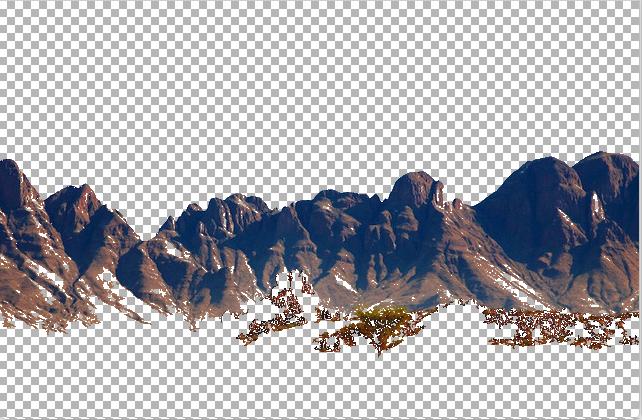
\includegraphics[width=7cm]{Figures/results/euclidean/img4/cluster2.png} }}
	\subfloat[Segment 3]{{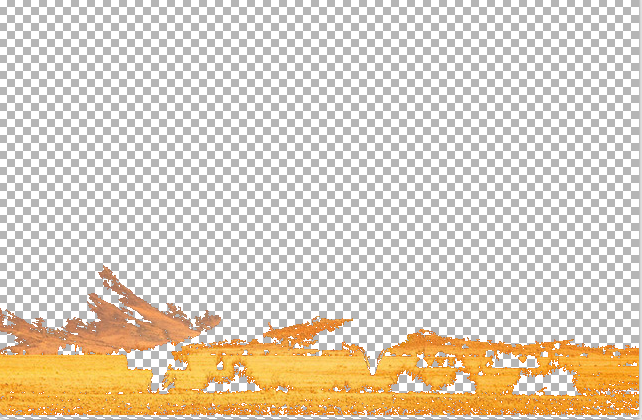
\includegraphics[width=7cm]{Figures/results/euclidean/img4/cluster3.png} }}
	\caption{Seed-Growing segmentace}
\end{figure}
\begin{figure}[H]
	\centering	
	\qquad
	\subfloat[Originál]{{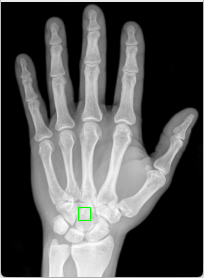
\includegraphics[height=5cm]{Figures/results/euclidean/img5/original.png} }}
	\subfloat[Segment 1]{{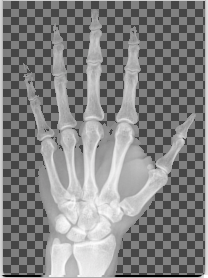
\includegraphics[height=5cm]{Figures/results/euclidean/img5/cluster1.png} }}
	\caption{Seed-Growing segmentace}
\end{figure}
\subsection{Geodetická vzdálenost}
Na následujích obrázcích se pokusíme ukázat zajímavé výsledky pomocí geodetické vzdálenosti, především schopnost algoritmu zpracovávat přechody v obraze.
\begin{figure}[H]
	\centering	
	\subfloat[Originál]{{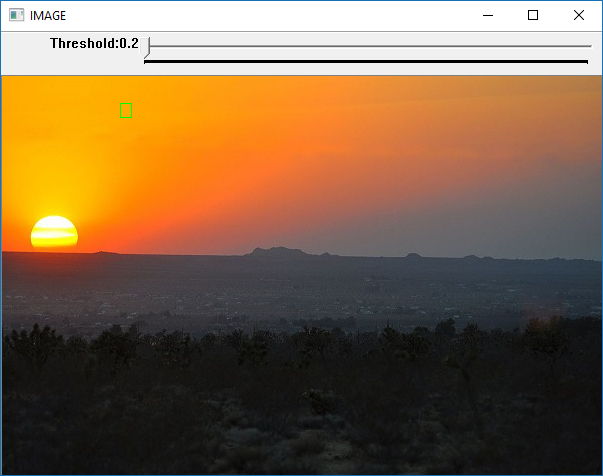
\includegraphics[width=7cm]{Figures/results/geodesic/img3/original.png} }}
	\subfloat[Segment 1]{{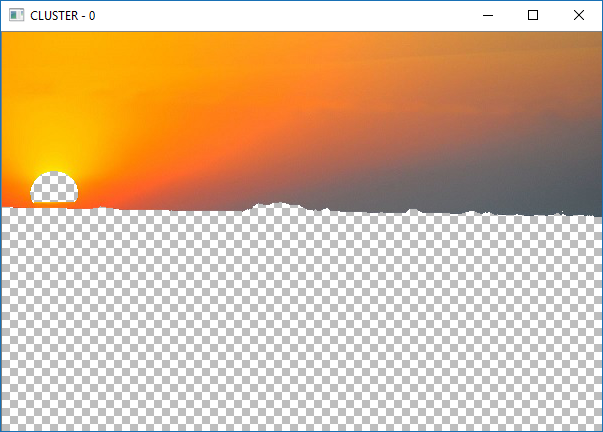
\includegraphics[width=7cm]{Figures/results/geodesic/img3/cluster0.png} }}
	\qquad
	\subfloat[Originál]{{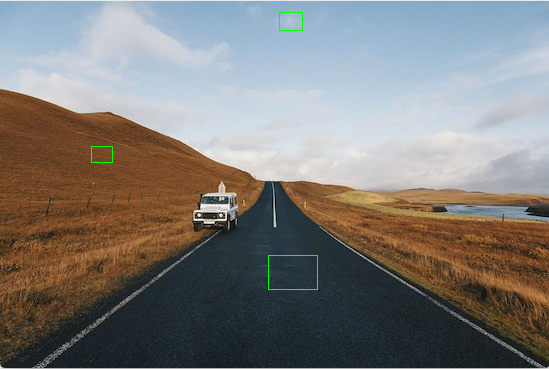
\includegraphics[width=7cm]{Figures/results/geodesic/img2/original.png} }}
	\subfloat[Segment 1]{{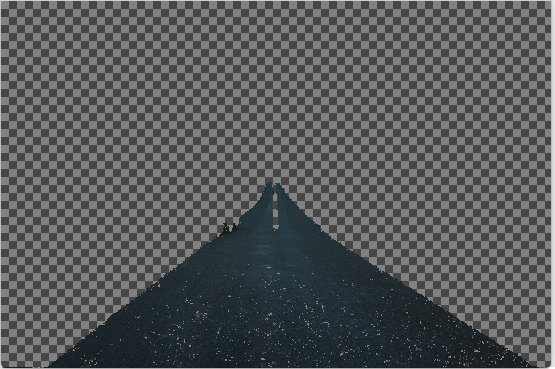
\includegraphics[width=7cm]{Figures/results/geodesic/img2/cluster2.png} }}
	\qquad
	\subfloat[Originál]{{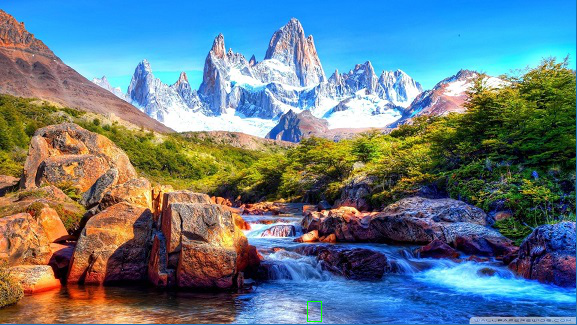
\includegraphics[width=7cm]{Figures/results/geodesic/img1/original.png} }}
	\subfloat[Segment 1]{{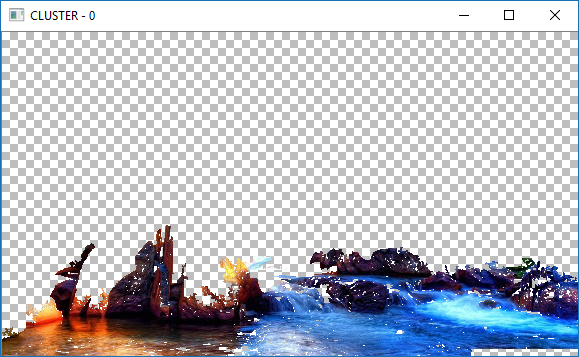
\includegraphics[width=7cm]{Figures/results/geodesic/img1/cluster1.png} }}
	\caption{Segmentace pomocí geodetické vzdálenosti}
\end{figure}
\newpage
\subsection{Rezistivní vzdálenost}
\begin{figure}[H]
	\centering	
	\subfloat[Originál]{{\includegraphics[width=5cm]{Figures/results/resistance/img1/original.png} }}
	\subfloat[Segment 1]{{\includegraphics[width=5cm]{Figures/results/resistance/img1/cluster1.png} }}
	\subfloat[Segment 2]{{\includegraphics[width=5cm]{Figures/results/resistance/img1/cluster2.png} }}
\qquad
	\subfloat[Originál]{{\includegraphics[width=5cm]{Figures/results/resistance/img2/original.png} }}
	\subfloat[Segment 1]{{\includegraphics[width=5cm]{Figures/results/resistance/img2/cluster1.png} }}
	\subfloat[Segment 2]{{\includegraphics[width=5cm]{Figures/results/resistance/img2/cluster2.png} }}
	\caption{Segmentace pomocí rezistivní vzdálenosti}
\end{figure}
\subsection{Doby segmentace}
Následující graf ukazuje naměřené doby segmentace. Z dat lze vidět chování a složitost jednotlivých metod segmentace. Měření bylo provedeno na procesoru (Core i7-6700, 3.40Ghz).
\newline
\newline
\newline
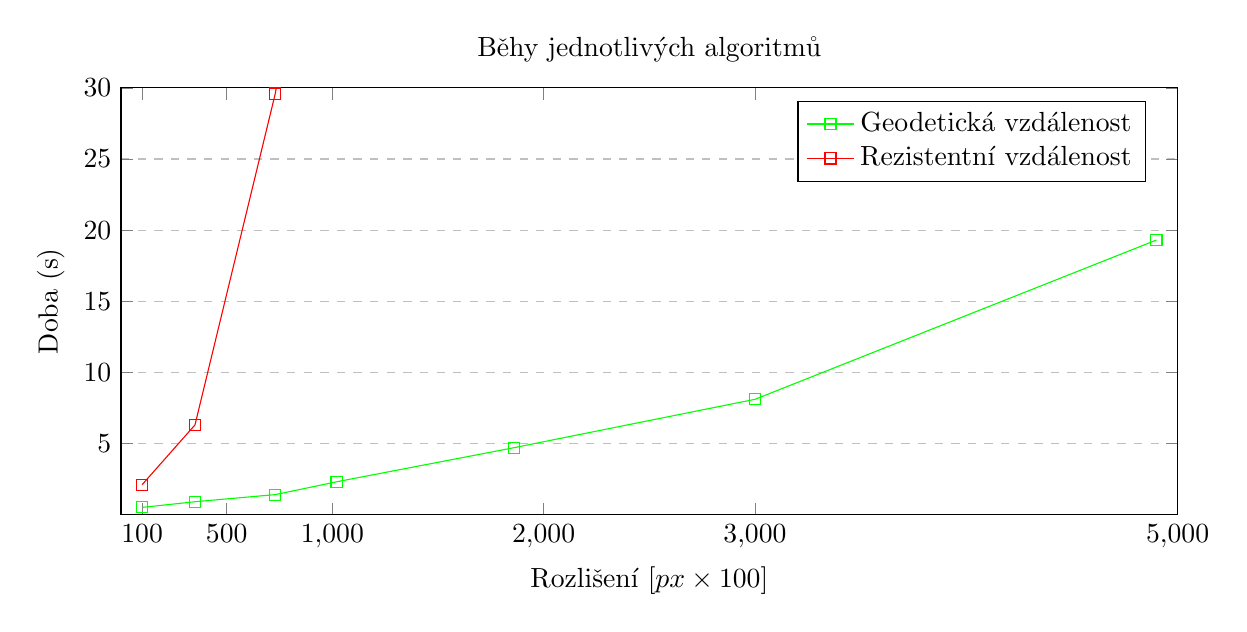
\begin{tikzpicture}

\begin{axis}
[
width=15cm,
height=7cm,
title={Běhy jednotlivých algoritmů},
ylabel={Doba (s)},
xlabel={Rozlišení [$px \times 100$]},
ymin=0, ymax=30,
xmin=0, xmax=5000,
ytick={5, 10, 15, 20, 25, 30, 45, 60},
xtick={100, 500, 1000, 2000, 3000, 5000},
legend pos=north east,
ymajorgrids=true,
grid style=dashed,
]

\addplot[
color=green,
mark=square,
]
coordinates {
	(100,0.5)(350,0.9)(730,1.4)(1020,2.3)(1860,4.7)(3000,8.1)(4900,19.3)
};

\addplot[
color=red,
mark=square,
]
coordinates {
	(100,2.1)(350,6.3)(730,29.6)(1020,56)
};
\legend{Geodetická vzdálenost, Rezistentní vzdálenost}

\end{axis}
\end{tikzpicture}

\section*{Závěr}
Cílem práce bylo porovnat různé způsoby měření vzdáleností při použití v algoritmech obrazové segmentace. Zaměřili jsme se především na metody jako jsou geodetická a rezistivní vzdálenost. Následně jsme experimentálně porovnali metody s běžnými shlukovacími algoritmy využívající růst regionů a euklidovskou vzdálenost. Ačkoliv je euklidovská vzdálenost často používaným řešení pro vyčíslování podobnosti mezi objekty, experimentálně jsme ukázali jasné nedostatky této metody, především při najivním způsobu segmentace.\par
První ověřenou metodou měření byla geodetická vzdálenost, hledající nejkratší cestu v grafu. Pro nalezení nejkratší cesty v obrazovém grafu jsme použili Dijsktrův algoritmus. Výsledky na jasně ukázali lepší segmentaci, především v částech s plynulou změnou jasu. Nevýhodou této metody je fakt, že i jedna nekonečně malá cesta nízkého konstrastu způsobí, zařazení objektu do segmentu, ignorující možnost vzniku dané cesty signálovým šumem. Ne jen kvalita rozpoznání objektů, ale i rychlost výpočtu a paměťové nároky jsou důležitým faktorem. Segmentaci pomocí geodetické vzdálenosti bych nazval jako středně rychlou. Algoritmus je pomalejší než segmentace pomocí euklidovské vzdálenosti. Nicméně mnohem rychlejší, než výpočet soustavy rovnic u vzdálenosti rezistivní.\par
Poslední porovnávanou metodou byla rezistivní vzdálenost. Osobně vidím její praktickou aplikaci jako velice komplikovanou a pro obrazovou segmentaci nevhodnou. Jasnou nevýhodou jsou vysoké paměťové nároky při výpočtu Laplaceovy matice z obrazového grafu. Samotné výsledky segmentace nejsou taktéž nijak uspokojující. Definovaná vzdálenost se dá popsat jako souhrnná vzdálenost všech cest v obrazovém grafu. Dle mého názoru je tato vlastnost velice nevhodná, jelikož na reálných obrazech často exitují situace kde se dva segmenty částečně prolínají. Současně hrozí situace, kdy se oba měřené body nacházejí na homogenní ploše což vede k vypočtení maximální vodivosti nevhodnému rozložení potenciálů v grafu. \par
Řešení problému geodetické a rezistivní vzdálenosti věnuje podstatnou část své dizertační práce Jan Gaura, kde představil kombinaci těchto dvou metod v podobě Rezistentně-Geodetické vzdálenosti.\cite{Gaura} Ta se pokouší využití nejlepších vlastností obou těchto metod a eliminovat jejich nedostatky.\par
Segmentace obrazu je jistě velkým problémem. Z pohledu technologického vývoje v oblasti automazatice a umělé inteligence se dá předpokládat, že pokrok v této oblasti bude pokračovat. Hardwarové požadavky byly ještě před pár lety příliš vysoké na implementování těchto algoritmů do zařízení bežného života. V posledních letech embedded systémy zaznamenaly velký výkonový nárůst, ať už v podobně grafických modulů nebo programovatelných FPGA čipů. Je tedy pravděpodobné, že se s inteligentními zařízeními, využívající v nějaké míře právě algoritmy obrazové segmentace budeme v běžném životě setkávat stále častěji.

\pagestyle{plain}
\begin{thebibliography}{99}	
	\pagenumbering{gobble}
	\bibitem{Sojka}SOJKA, Eduard. Digitální zpracování a analýza obrazů. Ostrava: VŠB-Technická univerzita, 2000. ISBN 80-7078-746-5.
	\bibitem{Cima}CIMA, Vojtěch. Segmentace obrazu metodou spektrálního a difůzního spektrálního shlukování. Ostrava: VŠB-Technická univerzita, 2015. Diplomová práce.
	\bibitem{Bayer}BAYER, E. Bryce. Color imaging array. 1976. US Patent 3,971,065
	\bibitem{Shlukovani} LUKASOVÁ, Alena a Jana ŠARMANOVÁ. Metody shlukové analýzy. Praha: Státní nakladatelství technické literatury, 1985.
	\bibitem{Kumar} KUMAR, Vipin, Introduction to Dataming - Chapter 8. Cluster Analysis: Basic Concepts and Algorithms
	\bibitem{Gaura} GAURA, Jan. SOJKA, Eduard. Diffusion-based Image Segmentation Methods. 2012.
	\bibitem{Berkeley} ONLINE, The Berkeley Segmentation Dataset and Benchmark
	\bibitem{Kleinberg} KLEINSBER, Jon. An Imposibility Theorem for Clustering. 2002
	\bibitem{Mumford} MUMFORD, D., SHAH, J.: Optimal Approximations by piece-wise Smooth Functions and Associated Variational Problems, Communications on Pure Applied Mathematics, 42, pp. 577-685, (1989) 
	\bibitem{Pecha}PECHA Marek. Segmentace obrazu s využitím spektrálníh shlukování. Ostrava: VŠB-Technická univerzita, 2014. Bakalářská práce.
	\bibitem{Dass} DASS Rajeshwar, PRIYANKA, DEVI Swapna, Image segmentation techniques
	\bibitem{Canny} CANNY, FRANCIS John, Finding Edges and Lines in Images, 1983
	\bibitem{Zelnik} ZELNIK, MANOR, L., PERONA, P.: Self-Tuning Spectral Clustering, Advances in Neural Information Processing Systems, 17, pp. 1601-1608, (2004)
	\bibitem{Jordan} Ng, A., Jordan, M., and Weiss, Y.: On Spectral Clustering: Analysis and an Algorithm, Advances in Neural Information Processing Systems, 14, pp. 849-856, (2002)
	\bibitem{Dostal}DOSTÁL Zdeněk, VONDRÁK Vít, Lineární algebra. Skripta VŠB-TU Ostrava, 2000
	\bibitem{Algfoor}ALGFOOR ZA., SUNAR MS., HOLIVAND H, A Comprehensive Study on Pathfinding Techniques for Robotics and Video Games, International Journal of Computer Games Technology, vol. 2015, Article ID 736138, 2015.
	\bibitem{Bouttier} BOUTTIER J. FRANCESCO Di P., GUITTER E., Geodesic distance in planar graphs, Service de Physique Théorique, CEA/DSM/SPhT, Unité de recherche associée au CNRS, CEA/Saclay, 91191 Gif-sur-Yvette cedex, France 2003
	\bibitem{Kolar} KOLÁŘ, Josef. Teoretická informatika. 2. vyd. Praha : Česká informatická společnost, 2004. 205 s. ISBN 80-900853-8-5.
	\bibitem{Klein} Klein, D., J., Randic, M.: Resistance Distance, Journal of Mathematical Chemistry, 12, pp. 81-95, (1993)
	\bibitem{Babic} Babic, D., Klein, D., J., Lukovits, I., Nikolic, S., Trinajstic, N.: Resistance-Distance Matrix: A Computational Algorithm and Its Applications, International Journal of Quantum Chemistry, 90, pp. 166-176, (2002)
\end{thebibliography}

\appendix

\section{Diagram tříd}

\begin{figure}[H]
	\centering
	\includegraphics[width=10cm]{Figures/explanatory/appClassDiagram.png}
\end{figure}

\section{Výsledky}
\pagenumbering{roman}
\begin{figure}[H]
	\vspace*{+3.0mm}
	\centering
	\includegraphics[width=13cm]{Figures/results/euclidean/img1/original.png}
\end{figure}
\begin{figure}[H]
	\vspace*{+3.0mm}
	\centering
	\includegraphics[width=13cm]{Figures/results/euclidean/img1/cluster0.png}
\end{figure}
\begin{figure}[H]
	\vspace*{+3.0mm}
	\centering
	\includegraphics[width=13cm]{Figures/results/euclidean/img1/cluster1.png}
\end{figure}
\begin{figure}[H]
	\vspace*{+3.0mm}
	\centering
	\includegraphics[width=13cm]{Figures/results/euclidean/img1/cluster2.png}
\end{figure}

\begin{figure}[H]
	\vspace*{+3.0mm}
	\centering
	\includegraphics[width=13cm]{Figures/results/euclidean/img2/original.png}
\end{figure}
\begin{figure}[H]
	\vspace*{+3.0mm}
	\centering
	\includegraphics[width=13cm]{Figures/results/euclidean/img2/cluster0.png}
\end{figure}
\begin{figure}[H]
	\vspace*{+3.0mm}
	\centering
	\includegraphics[width=13cm]{Figures/results/euclidean/img2/cluster1.png}
\end{figure}
\begin{figure}[H]
	\vspace*{+3.0mm}
	\centering
	\includegraphics[width=13cm]{Figures/results/euclidean/img2/cluster2.png}
\end{figure}

\begin{figure}[H]
	\vspace*{+3.0mm}
	\centering
	\includegraphics[width=13cm]{Figures/results/geodesic/img3/original.png}
\end{figure}
\begin{figure}[H]
	\vspace*{+3.0mm}
	\centering
	\includegraphics[width=13cm]{Figures/results/geodesic/img3/cluster0.png}
\end{figure}

\section{Příloha na DVD}
Přiložené DVD obsahuje:
\begin{itemize}
	\item Multiplatformní aplikaci použitou pro experiment.
	\item Zdrojové kody k aplikaci.
	\item Technická dokumentace k aplikaci
	\item Zkompilované OpenCV knihovny pro všechny platformy.
	\item Sada testovacích obrázků.
\end{itemize}

\end{document}
